% !TEX program = xelatex
% !TEX encoding = UTF-8
%
% 석사학위논문 — 갑상선 결절 초음파 영상의 경량 검출·분할 모델
% 컴파일: XeLaTeX (한글 때문에 pdfLaTeX 불가) → BibTeX → XeLaTeX ×2
%         latexmk 사용 시 latexmkrc 가 자동으로 XeLaTeX 를 고른다.
%
% 표(tables/)와 그림(figures/)은 scripts/make_thesis.py 가 실험 결과에서 자동 생성한다.
% 본문(front/, chapters/, back/)은 직접 고치는 파일이다.

\documentclass[11pt,a4paper,oneside,openany]{report}

% ── 논문 정보: 여기만 고치면 표지·인준지·초록에 모두 반영된다 ───────────────
\newcommand{\ThesisTitleKo}{갑상선 결절 초음파 영상의 경량 검출·분할 모델}
\newcommand{\ThesisSubtitleKo}{추론 비용 없는 경계 정교화 모듈과 INT8 양자화를 중심으로}
\newcommand{\ThesisTitleEn}{A Lightweight Detection and Segmentation Model for Thyroid Nodules in Ultrasound Images}
\newcommand{\ThesisSubtitleEn}{Zero-Inference-Cost Boundary Refinement and INT8 Quantization}
\newcommand{\AuthorKo}{\fillin{홍길동}}
\newcommand{\AuthorEn}{\fillin{Gil-Dong Hong}}
\newcommand{\AdvisorKo}{\fillin{○○○}}
\newcommand{\AdvisorEn}{\fillin{Prof. ○○○}}
\newcommand{\UniversityKo}{\fillin{○○대학교}}
\newcommand{\UniversityEn}{\fillin{○○ University}}
\newcommand{\DepartmentKo}{\fillin{○○학과}}
\newcommand{\DepartmentEn}{\fillin{Department of ○○}}
\newcommand{\SubmitDate}{\fillin{2026년 12월}}
\newcommand{\DegreeDate}{\fillin{2027년 2월}}
\newcommand{\DegreeDateEn}{\fillin{February 2027}}

% ============================================================================
% 서식 설정 — main.tex 에서 \input 한다.
% ============================================================================
\usepackage{iftex}
\ifXeTeX\else\ifLuaTeX\else
  \errmessage{이 문서는 한글 조판 때문에 XeLaTeX(권장) 또는 LuaLaTeX로 컴파일해야 합니다.}
\fi\fi

% ── 한글 ────────────────────────────────────────────────────────────────
\usepackage{kotex}
\usepackage{fontspec}
% 설치된 글꼴을 순서대로 찾는다: Noto CJK(Overleaf·대부분 리눅스) → 나눔 → 은(TeX Live 기본)
\IfFontExistsTF{Noto Serif CJK KR}{\setmainhangulfont{Noto Serif CJK KR}[AutoFakeSlant=0.15]}{%
  \IfFontExistsTF{NanumMyeongjo}{\setmainhangulfont{NanumMyeongjo}[AutoFakeSlant=0.15]}{\setmainhangulfont{UnBatang}[AutoFakeSlant=0.15]}}
\IfFontExistsTF{Noto Sans CJK KR}{\setsanshangulfont{Noto Sans CJK KR}}{%
  \IfFontExistsTF{NanumGothic}{\setsanshangulfont{NanumGothic}}{\setsanshangulfont{UnDotum}}}
\IfFontExistsTF{Noto Sans Mono CJK KR}{\setmonohangulfont{Noto Sans Mono CJK KR}}{%
  \IfFontExistsTF{NanumGothicCoding}{\setmonohangulfont{NanumGothicCoding}}{\setmonohangulfont{UnDotum}}}

% ── 쪽 ──────────────────────────────────────────────────────────────────
\usepackage[a4paper,top=30mm,bottom=30mm,left=30mm,right=25mm,headheight=14pt]{geometry}
\usepackage{setspace}
\setstretch{1.55}
\setlength{\parindent}{1em}
\setlength{\parskip}{0.25em}
\usepackage{fancyhdr}
\pagestyle{plain}

% ── 수식·표·그림 ────────────────────────────────────────────────────────
\usepackage{amsmath,amssymb,mathtools,bm}
\usepackage{graphicx}
\graphicspath{{figures/}}
\usepackage{booktabs,multirow,array}
\usepackage{adjustbox}
\usepackage{float}
\usepackage[labelsep=period,font=small,labelfont=bf,skip=6pt]{caption}
\usepackage{subcaption}
\usepackage[section]{placeins}   % 절 경계를 넘어 그림·표가 떠다니지 않게
\usepackage{algorithm}
\usepackage{algpseudocode}
\usepackage{enumitem}
\setlist{itemsep=0.15em,topsep=0.4em,leftmargin=1.6em}
\usepackage{xcolor}
\usepackage{url}

% ── 참고문헌·링크 ──────────────────────────────────────────────────────
\usepackage[numbers,sort&compress]{natbib}
\setlength{\bibsep}{0.3em}
\usepackage[unicode,hidelinks,bookmarksnumbered]{hyperref}

% ── 장·절 제목 ─────────────────────────────────────────────────────────
\usepackage{titlesec}
\titleformat{\chapter}[display]{\centering\bfseries}{\Large 제\,\thechapter\,장}{0.5em}{\LARGE}
\titlespacing*{\chapter}{0pt}{0pt}{2.2em}
\titleformat{\section}{\bfseries\large}{\thesection}{0.8em}{}
\titleformat{\subsection}{\bfseries\normalsize}{\thesubsection}{0.8em}{}
\titlespacing*{\section}{0pt}{1.4em}{0.6em}
\titlespacing*{\subsection}{0pt}{1.0em}{0.4em}
\setcounter{secnumdepth}{2}
\setcounter{tocdepth}{2}

% ── 한국어 명칭 (kotex 가 문서 시작 때 덮어쓰지 않도록 \AtBeginDocument 에서 설정) ──
\AtBeginDocument{%
  \renewcommand{\contentsname}{목\quad 차}%
  \renewcommand{\listfigurename}{그림 목차}%
  \renewcommand{\listtablename}{표 목차}%
  \renewcommand{\bibname}{참고문헌}%
  \renewcommand{\figurename}{그림}%
  \renewcommand{\tablename}{표}%
  \renewcommand{\appendixname}{부록}%
}
\floatname{algorithm}{알고리즘}
\algrenewcommand\algorithmicrequire{\textbf{입력:}}
\algrenewcommand\algorithmicensure{\textbf{출력:}}
% 부록 장 제목은 '부록 A'
\usepackage{etoolbox}
\apptocmd{\appendix}{%
  \titleformat{\chapter}[display]{\centering\bfseries}{\Large 부록\,\thechapter}{0.5em}{\LARGE}}{}{}

% ── 본문용 매크로 ──────────────────────────────────────────────────────
\newcommand{\fillin}[1]{\textcolor{red}{#1}}            % 저자가 채울 자리 (최종본에서 빨간색 확인)
\newcommand{\TODO}[1]{\textcolor{red}{[확인 필요: #1]}}  % 저자가 확인해야 할 서술
\DeclareRobustCommand{\figref}[1]{그림~\ref{#1}}
\DeclareRobustCommand{\tabref}[1]{표~\ref{#1}}
\DeclareRobustCommand{\secref}[1]{\ref{#1}절}
\DeclareRobustCommand{\chapref}[1]{제\ref{#1}장}
\DeclareRobustCommand{\eqnref}[1]{식~(\ref{#1})}
\DeclareRobustCommand{\algref}[1]{알고리즘~\ref{#1}}
\DeclareRobustCommand{\appref}[1]{부록~\ref{#1}}
\newcommand{\BRM}{SegmentBRM}
\newcommand{\mAP}{mAP$_{50:95}$}
\newcommand{\tn}{TN3K}
\newcommand{\dd}{DDTI}
\newcommand{\todir}{$\rightarrow$}
\DeclareMathOperator*{\argmax}{arg\,max}
\DeclareMathOperator{\BCE}{BCE}
\DeclareMathOperator{\dil}{dilate}
\DeclareMathOperator{\ero}{erode}


\begin{document}

% ── 앞부분 (로마 숫자 쪽번호) ─────────────────────────────────────────
\pagenumbering{roman}
% 표지 — 학교 양식이 정해져 있으면 그 양식에 맞춰 이 파일만 바꾸면 된다.
\begin{titlepage}
\begin{center}
\vspace*{8mm}
{\large 공학석사 학위논문\par}
\vspace{30mm}
{\LARGE\bfseries\ThesisTitleKo\par}
\vspace{5mm}
{\Large --- \ThesisSubtitleKo\ ---\par}
\vspace{12mm}
{\large \ThesisTitleEn\par}
\vspace{2mm}
{\normalsize \ThesisSubtitleEn\par}
\vfill
{\large \DegreeDate\par}
\vspace{14mm}
{\large \UniversityKo\ 대학원\par}
\vspace{2mm}
{\large \DepartmentKo\par}
\vspace{8mm}
{\Large \AuthorKo\par}
\vspace*{10mm}
\end{center}
\end{titlepage}

% 속표지 (지도교수·제출 문구)
\begin{titlepage}
\begin{center}
\vspace*{20mm}
{\LARGE\bfseries\ThesisTitleKo\par}
\vspace{5mm}
{\Large --- \ThesisSubtitleKo\ ---\par}
\vspace{30mm}
{\large 지도교수\quad \AdvisorKo\par}
\vspace{20mm}
{\large 이 논문을 공학석사 학위논문으로 제출함\par}
\vspace{4mm}
{\large \SubmitDate\par}
\vfill
{\large \UniversityKo\ 대학원\par}
\vspace{2mm}
{\large \DepartmentKo\par}
\vspace{8mm}
{\Large \AuthorKo\par}
\vspace*{10mm}
\end{center}
\end{titlepage}

% 인준지 — 심사위원 서명란. 학교 양식이 있으면 교체한다.
\begin{titlepage}
\begin{center}
\vspace*{30mm}
{\Large\bfseries \AuthorKo 의 공학석사 학위논문을 인준함\par}
\vspace{40mm}
\renewcommand{\arraystretch}{2.6}
\begin{tabular}{l p{55mm} l}
심사위원장 & \hrulefill & (인) \\
심사위원   & \hrulefill & (인) \\
심사위원   & \hrulefill & (인) \\
\end{tabular}
\vfill
{\large \UniversityKo\ 대학원\par}
\vspace{4mm}
{\large \DegreeDate\par}
\vspace*{10mm}
\end{center}
\end{titlepage}

% 국문 초록
\chapter*{국문 초록}
\phantomsection\addcontentsline{toc}{chapter}{국문 초록}

\begin{center}
{\large\bfseries \ThesisTitleKo\par}
{\normalsize --- \ThesisSubtitleKo\ ---\par}
\vspace{2mm}
{\normalsize \AuthorKo\quad \DepartmentKo\ \UniversityKo\ 대학원\par}
\end{center}
\vspace{4mm}

갑상선 결절의 초음파 판독에서 결절의 경계(margin)는 악성도를 가늠하는 독립적인 채점 항목이다.
따라서 자동 분할 모델에 요구되는 것은 영역이 대체로 맞는 것을 넘어 경계가 정확한 것이며,
검진 현장이나 휴대형 초음파처럼 GPU가 없는 환경에서도 동작해야 실제로 쓰일 수 있다.
본 연구는 YOLOv11-seg를 기반으로, 두 공개 데이터셋을 혼합한 학습, 추론 비용을 늘리지 않는
경계 정교화, 사후 양자화를 통한 경량화를 하나의 파이프라인에서 검증하였다.

먼저 TN3K와 DDTI를 합친 4,130장(결절 4,457개)에 대해 출처 계층화 5-fold 교차검증과
학습에 쓰지 않은 TN3K test 614장의 held-out 평가, 그리고 한 데이터셋으로 학습해 다른 데이터셋에서
평가하는 LODO(leave-one-dataset-out) 실험을 설계하였다. 이 조건에서 YOLOv11n-seg(nano)는
small 모델보다 파라미터가 3.5배 적음에도 Mask \mAP{} 0.6272로 small(0.6239)과 동등하여
경량 모델을 기준 모델로 선택하였다.

다음으로 분할 헤드의 프로토타입 특징에서 갈라지는 학습 전용 경계 분기(\BRM{})와,
정답 마스크의 형태학적 경계 밴드에 가중치를 주는 경계 인식 손실을 제안하였다.
경계 분기는 4,657개의 파라미터(전체의 0.16\%)만 추가하며 추론 시에는 실행되지 않으므로
배포되는 연산 그래프는 베이스라인과 동일하다(9.73 GFLOPs). 손실 계수를 스윕으로 정한 뒤
held-out 평가에서 Dice는 0.8195에서 0.8300으로, HD95는 영상 대각선 대비 9.628\%에서 8.378\%로
13.0\% 개선되었고, Boundary IoU도 0.4358에서 0.4414로 향상되었다. 영상 단위 대응표본 검정(n=614)에서
세 지표 모두 유의하였다(Wilcoxon $p$ = 0.014, 0.0045, 0.011). 반면 교차 데이터셋 조건에서는 개선이
유지되지 않았으며, 3개 시드로 반복한 결과 악화 역시 통계적으로 확인되지 않아
일반화 여부는 판정할 수 없었다. 단일 시드 결과만으로는 큰 악화처럼 보였던 차이가
시드 반복 후 실행 간 변동 범위 안으로 들어왔다는 점도 함께 보고한다.

마지막으로 제안 모델을 ONNX FP32·FP16, ONNX Runtime 정적 INT8, OpenVINO INT8로 변환하여 비교하였다.
OpenVINO INT8 모델은 3.71 MB, CPU 지연 4.10 ms로 ONNX FP32(11.63 MB, 62.82 ms) 대비 15.3배 빨랐고,
Dice 0.8290으로 원본(0.8300)과 사실상 같은 정확도를 유지하였다. 같은 INT8이라도 ONNX Runtime에서는
검출 헤드를 부동소수점으로 남겨야 했기 때문에 44.00 ms에 그쳐, 양자화 효과가 변환 도구의
연산 선별 방식에 크게 좌우됨을 확인하였다.

\vspace{6mm}
\noindent\textbf{주요어}\quad 갑상선 결절, 초음파 영상, 인스턴스 분할, YOLOv11, 경계 정교화,
경계 인식 손실, 모델 경량화, 사후 양자화, 교차 데이터셋 일반화

\vspace{2mm}
\noindent\textbf{학\quad 번}\quad \fillin{○○○○-○○○○○}


\cleardoublepage
\phantomsection\addcontentsline{toc}{chapter}{\contentsname}
\tableofcontents
\cleardoublepage
\phantomsection\addcontentsline{toc}{chapter}{\listtablename}
\listoftables
\cleardoublepage
\phantomsection\addcontentsline{toc}{chapter}{\listfigurename}
\listoffigures

% ── 본문 (아라비아 숫자 쪽번호) ───────────────────────────────────────
\cleardoublepage
\pagenumbering{arabic}
% ============================================================================
\chapter{서론}\label{ch:intro}
% ============================================================================

\section{연구 배경}\label{sec:background}

갑상선 결절은 매우 흔한 소견이다. 고해상도 초음파를 사용하면 무작위로 선정한 성인의 19--68\%에서
결절이 발견되며, 그중 임상적으로 문제가 되는 갑상선암은 7--15\% 수준으로 보고된다\citep{haugen2016ata}.
발견되는 결절의 대부분이 양성이므로, 진료의 핵심은 어떤 결절에 세침흡인검사가 필요한지를
가려내는 데 있다. 이 판단의 1차 근거가 초음파 영상이다.

미국영상의학회의 ACR TI-RADS를 비롯한 주요 판독 체계는 결절의 구성, 에코, 형태, 경계(margin),
에코 발생 병소를 각각 채점하여 합산한다\citep{tessler2017tirads}. 이 가운데 경계는 독립된 채점
항목으로, 매끄럽거나 불분명한 경계에는 0점, 분엽상 또는 불규칙한 경계에는 2점,
갑상선 외 침범에는 3점이 부여된다. 경계 점수 하나가 결절의 위험 등급을 바꾸고 결과적으로
세침흡인검사 여부를 좌우할 수 있다. 다시 말해 갑상선 결절의 자동 분할에서 경계는 부수적인
정보가 아니라 판독 결과에 직접 들어가는 정보이다.

그러나 초음파 영상에서 경계를 정확히 그리는 일은 사람에게도 어렵다. 스페클 잡음, 결절 하방의
음향 음영, 주변 조직과의 낮은 대조도가 경계를 흐리게 만들고, 경계 관련 소견은 판독자 간
일치도가 낮은 항목으로 알려져 있다\citep{hoang2018interobserver}. 딥러닝 기반 자동 분할은
이 변이를 줄이고 판독 시간을 단축할 수단으로 연구되어 왔다\citep{ronneberger2015unet,gong2021multitask,gong2023trfe}.

자동 분할이 실제 진료에 들어가려면 정확도와 함께 배포 조건도 충족해야 한다. 건강검진 현장이나
휴대형 초음파 장비, 소규모 의원의 판독 PC에는 GPU가 없는 경우가 많다. 고성능 GPU 서버를
전제로 설계된 모델은 이런 환경에서 실시간으로 동작하지 못한다. 따라서 경계 정확도를 높이는
기법이 추론 비용을 늘린다면, 그 기법은 바로 이 배포 조건과 충돌하게 된다.

\section{문제 정의}\label{sec:problem}

본 연구는 위 배경에서 다음 세 가지 문제를 정의한다. 각 문제는 이후 실험 설계의 단계에 그대로
대응된다.

\paragraph{P1. 경계 품질은 영역 지표에 가려진다.}
분할 모델의 성능은 흔히 mAP나 IoU 같은 영역 중심 지표로 보고된다. 이 지표들은 결절 전체 면적에
대한 겹침을 재기 때문에, 면적에서 차지하는 비율이 작은 경계 부근의 몇 픽셀 오차에는 둔감하다.
경계가 실제로 나아졌는지 판정하려면 Boundary IoU\citep{cheng2021boundaryiou}나 95 백분위
Hausdorff 거리(HD95)\citep{taha2015metrics}처럼 경계에 특화된 지표로 함께 평가해야 한다.

\paragraph{P2. 공개 데이터셋은 서로 이질적이다.}
공개된 갑상선 초음파 데이터셋은 수집 기관, 장비, 화각, 주석 방식이 서로 다르다. 한 데이터셋에서
학습한 모델이 다른 데이터셋에서도 같은 성능을 낼지는 알 수 없으며, 의료영상 전반에서 이러한
도메인 이동은 성능 저하의 주된 원인으로 지적된다\citep{guan2022domain}. 여러 데이터셋을 혼합해
학습하고, 학습에 쓰지 않은 데이터셋에서 직접 평가하는 실험이 필요하다.

\paragraph{P3. 배포 환경에는 GPU가 없다.}
GPU 없이 CPU만으로 실시간 추론이 가능한 수준까지 모델의 크기와 연산량을 줄여야 한다.
이때 경량화가 P1에서 얻은 경계 품질을 훼손하지 않는지도 함께 확인해야 한다.

\section{연구 목적 및 가설}\label{sec:hypothesis}

본 연구의 목적은 갑상선 결절 초음파 영상에서 경계 정확도를 높이면서도 CPU에서 실시간으로
동작하는 검출·분할 모델을 만드는 것이다. 이를 위해 다음 세 가설을 세우고, 각 가설마다 검증 방법과
기각 조건을 미리 정하였다.

\begin{description}[leftmargin=2.2em,style=nextline]
  \item[H1 (모델 용량 가설)]
    YOLOv11-seg nano는 small보다 파라미터가 약 1/3.5임에도 갑상선 결절 검출·분할에서
    동등한 정확도를 낸다.\\
    \textit{검증}: 동일한 5-fold 분할과 학습 설정에서 두 모델을 학습하고 held-out 집합의
    Mask \mAP{}를 비교한다. \textit{기각 조건}: nano가 small보다 Mask \mAP{}에서
    fold 표준편차 이상 뒤처지는 경우.

  \item[H2 (경계 정교화 가설)]
    학습 시에만 동작하는 보조 경계 분기와 경계 가중 손실은 추론 비용을 전혀 늘리지 않고
    경계 품질을 개선한다.\\
    \textit{검증}: Dice, Boundary IoU, HD95를 영상 단위 대응표본 검정으로 비교하고, 배포 그래프의
    GFLOPs가 베이스라인과 같은지 확인한다. \textit{기각 조건}: 경계 지표의 개선이 유의하지 않거나
    추론 연산량이 증가하는 경우.

  \item[H3 (경량화 가설)]
    INT8 사후 양자화로 CPU 배포 요건을 만족시키면서 정확도 손실은 무시할 수 있는 수준으로
    유지된다.\\
    \textit{검증}: PyTorch, ONNX FP32·FP16, ONNX Runtime INT8, OpenVINO INT8의 다섯 정밀도에서
    정확도·크기·지연 시간을 비교한다. \textit{기각 조건}: CPU 지연이 실시간 기준에 못 미치거나
    Dice 손실이 fold 표준편차를 넘는 경우.
\end{description}

\section{연구의 기여}\label{sec:contribution}

본 연구의 기여는 다음과 같다.

\begin{enumerate}
  \item \textbf{추론 비용이 없는 경계 정교화.} 분할 헤드의 프로토타입 특징에서 갈라지는 학습 전용
    경계 분기와 형태학적 경계 밴드 기반 가중 손실을 제안하였다. 추가 파라미터는 4,657개이고
    추론 그래프는 베이스라인과 동일하며, held-out 평가에서 HD95를 13.0\% 줄였다.
  \item \textbf{경계 특화 평가와 통계 검정.} mAP에 드러나지 않는 경계 개선을 Boundary IoU와 HD95로
    측정하고, 평균 비교에 그치지 않고 영상 단위 대응표본 검정, 부트스트랩 신뢰구간,
    효과크기로 개선이 우연의 범위를 벗어나는지 확인하였다.
  \item \textbf{교차 데이터셋 결과의 신중한 보고.} 교차 데이터셋 실험을 3개 시드로 반복하여,
    단일 실행에서 크게 악화된 것처럼 보이던 차이가 실행 간 변동 범위 안에 있음을 보였다.
    또한 두 데이터셋의 정량적 차이(결절 수 분포, 결절 크기, 해상도)를 분석하여 교차 데이터셋
    성능이 낮은 원인을 데이터 측면에서 설명하였다.
  \item \textbf{배포 형식별 경량화 비교.} 같은 INT8이라도 변환 도구에 따라 CPU 지연이 44.00 ms와
    4.10 ms로 10배 이상 차이 남을 보이고, 그 원인을 양자화에서 제외되는 연산의 범위로 설명하였다.
    구현 과정에서 확인한 실패 사례(검출 헤드 양자화 시 출력 붕괴 등)도 함께 기록하였다.
\end{enumerate}

\section{논문의 구성}\label{sec:organization}

본 논문의 구성은 다음과 같다. \chapref{ch:related}에서는 의료영상 분할, 실시간 인스턴스 분할,
경계 정교화, 모델 경량화, 분할 평가 지표에 관한 선행연구를 정리하고 연구 공백을 도출한다.
\chapref{ch:dataset}에서는 사용한 두 데이터셋의 특성과 정량적 차이, 전처리와 분할 설계를 설명한다.
\chapref{ch:method}에서는 제안하는 경계 정교화 모듈과 경계 인식 손실, 학습--추론 분리 구조,
양자화 파이프라인을 기술한다. \chapref{ch:experiments}에서는 실험 설정과 결과를 가설 순서에 따라
제시하고, \chapref{ch:discussion}에서는 결과의 의미와 연구의 한계를 논의한다.
마지막으로 \chapref{ch:conclusion}에서 결론과 향후 연구 방향을 제시한다.

% ============================================================================
\chapter{관련 연구}\label{ch:related}
% ============================================================================

이 장에서는 본 연구와 관련된 다섯 갈래의 선행연구를 정리한다. 의료영상 분할의 기본 구조
(\secref{sec:rw_medseg}), 갑상선 결절 분할 연구와 공개 데이터셋(\secref{sec:rw_thyroid}),
실시간 인스턴스 분할(\secref{sec:rw_realtime}), 경계 정교화(\secref{sec:rw_boundary}),
모델 경량화와 양자화(\secref{sec:rw_quant})를 차례로 살펴보고, 평가 지표와 도메인 이동에 관한
논의(\secref{sec:rw_metric}, \secref{sec:rw_domain})를 거쳐 연구 공백을 도출한다(\secref{sec:rw_gap}).

\section{의료영상 분할}\label{sec:rw_medseg}

U-Net\citep{ronneberger2015unet}은 대칭적인 인코더--디코더와 같은 해상도끼리 특징을 잇는 스킵 연결로
적은 학습 데이터에서도 정밀한 분할을 가능하게 하여 의료영상 분할의 표준 구조가 되었다.
이후 중첩된 스킵 연결을 둔 UNet++\citep{zhou2018unetpp}, 데이터셋 특성에 맞춰 전처리와 구조를
자동으로 구성하는 nnU-Net\citep{isensee2021nnunet} 등이 제안되었으며, 영역 겹침을 직접 최적화하는
Dice 손실\citep{milletari2016vnet}도 널리 쓰인다.

이들은 영상 전체를 픽셀 단위로 분류하는 의미 분할(semantic segmentation) 모델이다. 한 영상에
결절이 여러 개 있을 때 각각을 구분하려면 별도의 후처리가 필요하고, 결절의 위치를 상자로
제시하는 검출 기능은 기본적으로 포함하지 않는다. 검출과 분할을 함께 수행하는 인스턴스 분할로는
Mask R-CNN\citep{he2017maskrcnn}이 대표적이지만, 2단계 구조여서 추론 비용이 크다.

\section{갑상선 결절 분할}\label{sec:rw_thyroid}

갑상선 결절 분할 연구는 공개 데이터셋의 등장과 함께 활발해졌다. DDTI\citep{pedraza2015ddti}는
콜롬비아의 영상센터에서 수집한 갑상선 초음파 영상과 판독 정보를 공개한 초기 데이터셋이다.
TN3K\citep{gong2021multitask}는 3,493장 규모의 갑상선 결절 분할 데이터셋으로, 이를 공개한 연구는
갑상선 영역 분할을 보조 과제로 두어 결절이 갑상선 안에 있다는 사전지식을 활용하는 다중 과제
학습을 제안하였다. 후속 연구인 TRFE-Net\citep{gong2023trfe}은 갑상선 영역 사전정보를 주의 기전으로
결절 분할에 주입하여 성능을 높였다.

이 연구들은 분할 정확도 향상에 초점을 두며, 모델의 경량화나 CPU 배포는 주된 관심사가 아니다.
또한 대부분 단일 데이터셋 안에서 학습과 평가를 수행하여, 서로 다른 데이터셋 사이의 일반화는
충분히 다뤄지지 않았다.

\section{실시간 인스턴스 분할}\label{sec:rw_realtime}

YOLO\citep{redmon2016yolo}는 검출을 단일 회귀 문제로 바꾸어 실시간 검출을 가능하게 하였다.
인스턴스 분할을 실시간으로 수행하는 방법으로는 YOLACT\citep{bolya2019yolact}가 중요한 전환점이다.
YOLACT는 영상 전체에 공유되는 소수의 프로토타입 마스크와, 검출된 객체마다 예측하는 마스크 계수를
분리하고, 둘의 선형 결합으로 객체별 마스크를 만든다. 마스크 생성이 행렬 곱 한 번으로 끝나므로
2단계 방식보다 훨씬 빠르다.

Ultralytics YOLOv8과 YOLOv11\citep{jocher2024yolo11}의 분할 모델은 이 프로토타입 방식을 따른다.
YOLOv11은 CSP 구조\citep{wang2020cspnet}를 경량화한 C3k2 블록, SPPF, 공간 주의 블록인 C2PSA를
백본에 두고, FPN\citep{lin2017fpn}·PAN\citep{liu2018panet} 형태의 넥에서 세 스케일의 특징을 융합한다.
검출 헤드는 앵커 없는(anchor-free) 방식으로 상자를 분포 형태로 회귀하는 DFL\citep{li2020gfl}과
과제 정렬 할당기\citep{feng2021tood}를 사용한다.

프로토타입 방식의 약점은 마스크 해상도이다. 프로토타입은 입력의 1/4 해상도에서 만들어지므로,
세밀한 경계를 표현하는 데 한계가 있고 경계가 거칠어지기 쉽다. 본 연구는 바로 이 지점을 개선
대상으로 삼는다.

\section{경계 정교화}\label{sec:rw_boundary}

분할 경계를 개선하는 방법은 크게 두 부류로 나뉜다.

\paragraph{추론 단계의 정교화.} PointRend\citep{kirillov2020pointrend}는 분할을 렌더링 문제로 보고,
불확실성이 높은 경계 부근의 점만 골라 고해상도 특징으로 반복 재분류한다. 경계 품질을 크게 높이지만,
추론 시 추가 모듈과 반복 연산이 필요하여 지연 시간이 늘어난다.

\paragraph{학습 단계의 경계 감독.} 손실 함수를 바꾸어 경계에 학습 신호를 집중시키는 방법이다.
Boundary loss\citep{kervadec2019boundary}는 정답 경계로부터의 거리 맵을 이용해 영역 적분 형태의
경계 손실을 정의하여 클래스 불균형이 심한 분할에서 효과를 보였다. Karimi와 Salcudean\citep{karimi2020hausdorff}은
Hausdorff 거리를 직접 줄이는 미분 가능한 손실을 제안하였다. 이 방법들은 추론 비용을 늘리지 않는다는
장점이 있으나, 대부분 픽셀 단위 의미 분할을 전제로 설계되어 프로토타입 기반 인스턴스 분할의
객체별 마스크 손실에 그대로 적용하기 어렵다.

본 연구는 두 번째 부류에 속하면서, 보조 경계 분기를 두어 공유 프로토타입 자체가 경계에 민감해지도록
학습시키되 그 분기를 추론 그래프에서는 완전히 제거하는 방식을 택한다.

\section{모델 경량화와 양자화}\label{sec:rw_quant}

모델 경량화 기법에는 가지치기, 지식 증류\citep{hinton2015distilling}, 경량 구조 설계, 양자화가 있으며
이들을 결합하기도 한다\citep{han2016deepcompression}. 이 가운데 양자화는 가중치와 활성값을 32비트
부동소수점에서 8비트 정수 등으로 낮추어 모델 크기와 연산량을 줄인다. Jacob 등\citep{jacob2018quantization}은
정수 연산만으로 추론하는 양자화 체계를 정립하였고, Krishnamoorthi\citep{krishnamoorthi2018whitepaper}와
Nagel 등\citep{nagel2021whitepaper}은 채널별 양자화, 캘리브레이션, 양자화 인식 학습 등 실무 지침을 정리하였다.

양자화는 재학습 없이 소량의 캘리브레이션 데이터로 변환하는 사후 양자화(PTQ)와 학습 중에 양자화
오차를 반영하는 양자화 인식 학습(QAT)으로 나뉜다. PTQ는 간편하지만 양자화에 민감한 연산이 있으면
정확도가 크게 떨어질 수 있어, 어떤 연산을 부동소수점으로 남길지가 결과를 좌우한다.
OpenVINO의 NNCF\citep{kozlov2020nncf}는 구조를 분석하여 민감한 연산을 양자화 범위에서 제외하는
기능을 제공한다.

\section{분할 평가 지표}\label{sec:rw_metric}

Dice 계수와 IoU는 영역 겹침을 재는 가장 일반적인 지표이다. 그러나 이들은 면적 전체에 대한 비율이므로
큰 객체에서 경계 부근 오차의 영향이 희석된다\citep{taha2015metrics}. Hausdorff 거리는 두 경계 사이의 최대
거리로 경계의 최악 오차를 직접 반영하며, 이상치에 대한 민감도를 낮추기 위해 95 백분위값(HD95)이 흔히
쓰인다. Boundary IoU\citep{cheng2021boundaryiou}는 두 마스크의 경계로부터 일정 폭 안의 띠 영역에서만 IoU를
계산하여, 객체 크기와 무관하게 경계 품질에 민감한 지표를 제공한다.

\section{의료영상의 도메인 이동}\label{sec:rw_domain}

의료영상 모델은 학습 데이터와 장비, 촬영 프로토콜, 환자군이 다른 데이터에서 성능이 떨어지는 경우가
많다\citep{guan2022domain}. 이를 완화하기 위해 도메인 적대 학습\citep{ganin2015dann} 등 도메인 적응 기법이
연구되고 있다. 한편 이러한 일반화 성능을 평가할 때는 실행 간 변동을 고려해야 한다. 같은 설정이라도
난수 시드에 따라 결과가 상당히 달라질 수 있어, 단일 실행으로 기법 간 우열을 판단하면 잘못된 결론에
이를 수 있다\citep{bouthillier2021variance}.

\section{연구 공백}\label{sec:rw_gap}

\tabref{tab:related}는 선행연구를 본 연구의 관점에서 요약한 것이다.

\begin{table}[htbp]
\centering\small
\caption{선행연구 요약과 본 연구의 위치.}
\label{tab:related}
\begin{tabular}{p{0.2\linewidth}p{0.33\linewidth}p{0.38\linewidth}}
\toprule
계열 & 대표 연구 & 본 연구와의 관계 \\
\midrule
의료영상 분할 & U-Net\citep{ronneberger2015unet}, UNet++\citep{zhou2018unetpp}, nnU-Net\citep{isensee2021nnunet}
  & 정확도는 높으나 검출·분할 통합과 추론 비용은 주된 관심이 아님 \\
갑상선 결절 분할 & TN3K\citep{gong2021multitask}, TRFE-Net\citep{gong2023trfe}, DDTI\citep{pedraza2015ddti}
  & 갑상선 영역 사전정보 활용. 경량화·교차 데이터셋 평가는 범위 밖 \\
실시간 인스턴스 분할 & YOLACT\citep{bolya2019yolact}, YOLOv11-seg\citep{jocher2024yolo11}
  & 빠르지만 1/4 해상도 프로토타입으로 경계가 거침 \\
경계 정교화 & PointRend\citep{kirillov2020pointrend}, Boundary loss\citep{kervadec2019boundary}, HD loss\citep{karimi2020hausdorff}
  & 추론 비용이 늘거나 의미 분할을 전제로 함 \\
양자화 & Jacob 등\citep{jacob2018quantization}, NNCF\citep{kozlov2020nncf}
  & 일반 기법. 분할 경계 품질에 미치는 영향은 별도 검증 필요 \\
평가 지표 & Boundary IoU\citep{cheng2021boundaryiou}, HD95\citep{taha2015metrics}
  & 본 연구의 주 평가 지표로 채택 \\
\bottomrule
\end{tabular}
\end{table}

정리하면, 갑상선 초음파 인스턴스 분할에서 \textbf{추론 비용을 늘리지 않는 경계 정교화}와
\textbf{CPU 배포를 위한 양자화}를 하나의 파이프라인에서 함께 검증하고, 그 효과를 경계 특화 지표와
통계 검정, 교차 데이터셋 실험으로 평가한 연구는 드물다. 본 연구는 이 공백을 다룬다.

% ============================================================================
\chapter{데이터셋}\label{ch:dataset}
% ============================================================================

본 연구는 서로 다른 기관과 장비에서 수집된 두 공개 데이터셋, TN3K와 DDTI를 함께 사용한다.
두 데이터셋을 의도적으로 혼합한 이유는 \secref{sec:problem}의 P2, 즉 데이터셋 간 이질성을 학습과 평가에
모두 반영하기 위해서이다. 이 장에서는 각 데이터셋의 특성(\secref{sec:ds_tn3k}, \secref{sec:ds_ddti}),
두 데이터셋의 정량적 차이(\secref{sec:ds_gap}), 전처리 절차(\secref{sec:ds_preproc}),
그리고 분할 설계(\secref{sec:ds_split})를 설명한다.

\section{TN3K}\label{sec:ds_tn3k}

TN3K\citep{gong2021multitask,gong2023trfe}는 갑상선 결절 초음파 영상 3,493장과 픽셀 단위 결절 마스크로
구성된 데이터셋이다. 배포 시 학습·검증용 2,879장과 평가용 614장으로 나뉘어 있으며, 본 연구는 이 구분을
그대로 따라 평가용 614장을 어떤 학습이나 모델 선택에도 사용하지 않는 held-out 집합으로 두었다.

\figref{fig:tn3k_samples}에서 보듯 TN3K 영상은 결절 주변을 잘라낸 확대 영상이 대부분이다.
그 결과 해상도가 184$\times$174부터 1463$\times$826까지 영상마다 제각각이며, 학습·검증 분할에서만
2,443종의 서로 다른 해상도가 나타난다. 판독 중 남긴 측정 커서(캘리퍼)가 영상에 그대로 찍혀 있는 경우도
있다. 한 영상에 결절이 둘 이상인 경우가 학습·검증 분할의 7.8\%, 평가 분할의 11.4\%를 차지한다.

\begin{figure}[htbp]
  \centering
  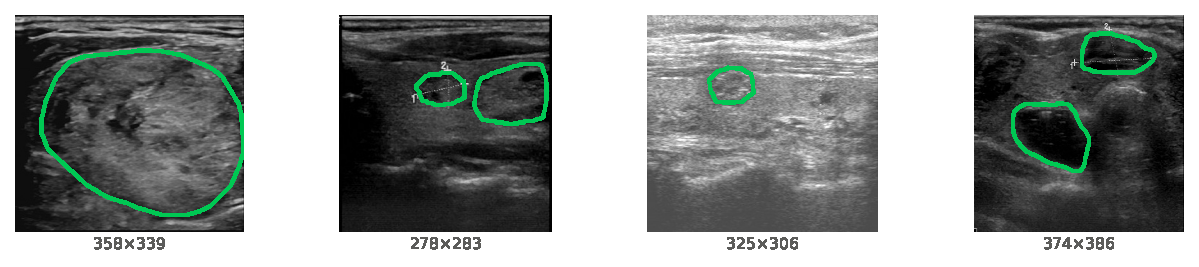
\includegraphics[width=\linewidth]{fig11_tn3k_samples}
  \caption[TN3K 표본과 정답 결절 경계(초록).]{TN3K 표본과 정답 결절 경계(초록). 각 영상 아래의 숫자는 원본 해상도이다.
    두 번째와 네 번째 영상에는 결절이 두 개씩 있다.}
  \label{fig:tn3k_samples}
\end{figure}

\section{DDTI}\label{sec:ds_ddti}

DDTI\citep{pedraza2015ddti}는 콜롬비아 IDIME 영상센터에서 수집한 갑상선 초음파 데이터셋이다.
본 연구에서는 결절 마스크가 제공되는 637장을 전부 학습·검증에 사용하였다.

DDTI 영상은 초음파 장비 화면을 그대로 캡처한 형태이다(\figref{fig:ddti_samples}). 그래서 영상 안에
게인 막대, 프로브 정보(P100, 12L6 등), 깊이 눈금, 좌우 표기(스페인어 DER·IZQ)가 함께 찍혀 있다.
높이는 모든 영상이 360 픽셀로 같고, 너비는 280, 560, 315, 245 픽셀의 네 종류뿐이다. 너비 560 픽셀 영상은
장비 화면 전체를, 280 픽셀 영상은 그중 초음파 영역 부근을 담고 있다. 637장 모두 결절이 정확히
하나씩이며, 다중 결절 사례는 하나도 없다.

\begin{figure}[htbp]
  \centering
  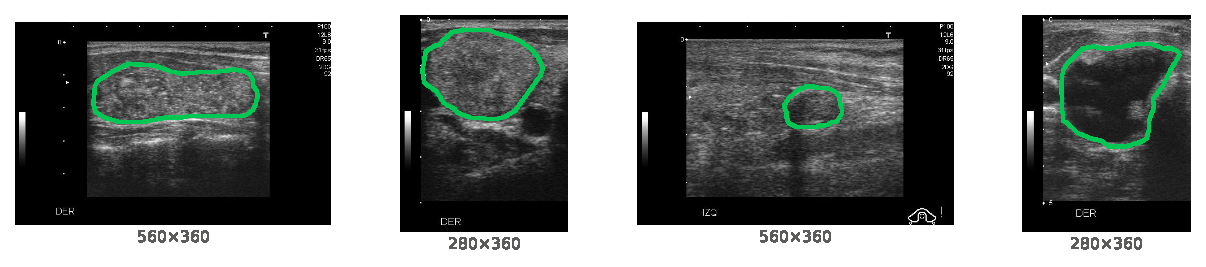
\includegraphics[width=\linewidth]{fig12_ddti_samples}
  \caption[DDTI 표본과 정답 결절 경계(초록).]{DDTI 표본과 정답 결절 경계(초록). 장비 화면의 게인 막대·눈금·좌우 표기가 영상에 포함되어 있다.}
  \label{fig:ddti_samples}
\end{figure}

\section{두 데이터셋의 정량적 차이}\label{sec:ds_gap}

\tabref{tab:dataset_stats}와 \figref{fig:dataset_stats}는 두 데이터셋의 차이를 정량적으로 보여 준다.
이 차이는 이후 교차 데이터셋 실험(\secref{sec:exp_lodo})의 설계 근거이자 그 결과를 해석하는 근거가 된다.

% 자동 생성 파일 — scripts/make_thesis.py 가 덮어쓴다. 직접 고치지 말 것.
\begin{table}[htbp]
\centering
\small
\caption[사용한 두 공개 데이터셋의 통계.]{사용한 두 공개 데이터셋의 통계. 결절 면적은 정답 폴리곤 면적을 영상 면적으로 나눈 값이다.}
\label{tab:dataset_stats}
\begin{adjustbox}{max width=\linewidth}
\begin{tabular}{lrrr}
\toprule
항목 & TN3K (trainval) & TN3K (test) & DDTI \\
\midrule
영상 수 & 2,879 & 614 & 637 \\
결절 수 & 3,130 & 690 & 637 \\
영상당 평균 결절 수 & 1.09 & 1.12 & 1.00 \\
결절 2개 이상 영상 비율 (\%) & 7.8 & 11.4 & 0.0 \\
파일 형식 & JPG & JPG & PNG \\
너비 범위 (px) & 184--1463 & 255--1399 & 245--560 \\
높이 범위 (px) & 174--826 & 261--772 & 360--360 \\
해상도 중앙값 (px) & 390$\times$336 & 436$\times$375 & 280$\times$360 \\
고유 해상도 종류 수 & 2,443 & 555 & 4 \\
결절 면적 중앙값 (영상 대비 \%) & 7.16 & 5.31 & 7.46 \\
결절 면적 5--95 백분위 (\%) & 0.88--42.95 & 0.59--37.33 & 1.52--23.76 \\
결절 면적 최솟값 (\%) & 0.056 & 0.162 & 0.524 \\
\bottomrule
\end{tabular}
\end{adjustbox}
\end{table}


\begin{figure}[htbp]
  \centering
  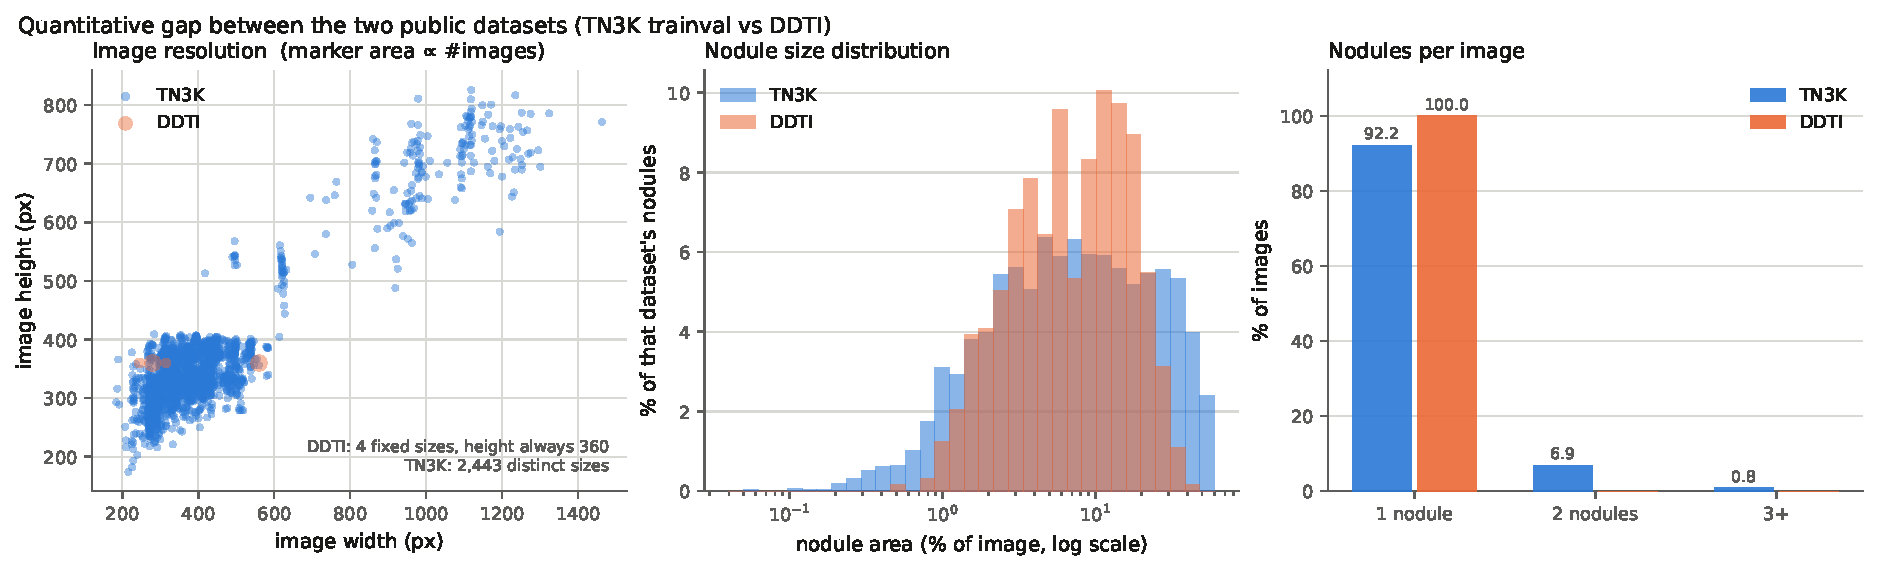
\includegraphics[width=\linewidth]{fig13_dataset_stats}
  \caption[두 데이터셋의 정량적 차이.]{두 데이터셋의 정량적 차이. (왼쪽) 영상 해상도 — 마커 넓이는 해당 해상도의 영상 수에 비례한다.
    (가운데) 결절 면적 분포 — 표본 수 차이를 없애기 위해 각 데이터셋 안에서의 비율로 정규화하였다.
    (오른쪽) 영상당 결절 수.}
  \label{fig:dataset_stats}
\end{figure}

\paragraph{해상도.} TN3K는 수천 종의 서로 다른 해상도를 가지는 반면 DDTI는 네 종류로 고정되어 있다.
학습 시에는 두 데이터셋 모두 640$\times$640 레터박스로 크기를 맞추지만, 원본에서 결절이 차지하는
픽셀 스케일의 분포는 크게 다르다.

\paragraph{결절 크기.} 결절 면적의 중앙값은 TN3K 7.16\%, DDTI 7.46\%로 비슷하지만 분포의 폭이 다르다.
TN3K는 영상의 0.06\%에 불과한 작은 결절부터 40\%를 넘는 큰 결절까지 넓게 퍼져 있는 반면, DDTI는
5--95 백분위가 1.52--23.76\%로 좁고 최솟값도 0.524\%이다. DDTI만으로 학습한 모델은 아주 작은 결절과
화면 대부분을 차지하는 큰 결절을 거의 본 적이 없다.

\paragraph{결절 수.} DDTI는 모든 영상이 단일 결절이다. DDTI로만 학습한 모델은 한 영상에 결절이 여럿 있는
장면을 학습하지 못하므로, TN3K로 옮겨 갔을 때 두 번째 결절을 놓칠 가능성이 높다.

\section{전처리}\label{sec:ds_preproc}

두 데이터셋은 정답을 비트맵 마스크로 제공한다. YOLOv11-seg는 객체마다 정규화된 다각형 좌표를 라벨로
받으므로, 마스크를 다각형으로 변환하였다. 두 데이터셋의 마스크는 JPEG 압축 잡음이 섞여 있거나
경계가 흐린 경우가 있어, 다음 절차를 두 데이터셋에 똑같이 적용하였다(\algref{alg:mask2poly}).

\begin{algorithm}[htbp]
\caption{정답 마스크의 YOLO-seg 다각형 변환}\label{alg:mask2poly}
\begin{algorithmic}[1]
\Require 마스크 영상 $M$ (높이 $h$, 너비 $w$)
\Ensure 정규화된 다각형 목록 $\mathcal{P}$
\State $B \gets [\,M > 127\,]$ \Comment{압축 잡음 제거를 위한 이진화}
\State $B \gets \mathrm{open}_{3\times3}(B)$ \Comment{모폴로지 열림으로 작은 잡티 제거}
\State $\mathcal{C} \gets$ 외곽 윤곽선 추출$(B)$ \Comment{내부 구멍은 무시}
\State $a_{\min} \gets \max(15,\ 0.0005\,hw)$
\For{각 윤곽선 $c \in \mathcal{C}$}
  \If{$\mathrm{area}(c) < a_{\min}$} \textbf{continue} \EndIf
  \State $c \gets$ Douglas--Peucker 단순화$(c,\ \varepsilon = 0.002 \cdot \mathrm{perimeter}(c))$
  \If{$|c| \ge 3$} $\mathcal{P} \gets \mathcal{P} \cup \{\, (x/w,\ y/h) \text{ for } (x,y) \in c \,\}$ \EndIf
\EndFor
\State \Return $\mathcal{P}$ \Comment{모든 다각형은 단일 클래스 `nodule'}
\end{algorithmic}
\end{algorithm}

최소 면적 기준(영상 면적의 0.05\%)은 마스크 잡티를 결절로 오인하지 않기 위한 것이다. 실제로 TN3K의 가장
작은 결절은 영상의 0.056\%로 이 기준을 넘는다. 변환 결과 TN3K 학습·검증 3,130개, TN3K 평가 690개,
DDTI 637개, 모두 4,457개의 결절 다각형을 얻었다. 변환된 다각형 전체를 원본 마스크 위에 겹쳐 그려
대조하였으며, 마스크가 있는데 라벨이 비거나 라벨이 누락된 영상은 없었다.

\section{분할 설계}\label{sec:ds_split}

실험의 목적에 따라 세 가지 분할을 구성하였다(\tabref{tab:splits}).

% 자동 생성 파일 — scripts/make_thesis.py 가 덮어쓴다. 직접 고치지 말 것.
\begin{table}[htbp]
\centering
\small
\caption[데이터 분할 구성.]{데이터 분할 구성. 괄호 안은 TN3K / DDTI 영상 수이다. pooled 5-fold의 평가는 모두 학습에 쓰이지 않은 TN3K test 614장에서 수행하였다.}
\label{tab:splits}
\begin{adjustbox}{max width=\linewidth}
\begin{tabular}{lrrrrr}
\toprule
분할 & 학습 & (TN3K / DDTI) & 검증 & (TN3K / DDTI) & 평가 \\
\midrule
fold 0 & 2,812 & 2,303 / 509 & 704 & 576 / 128 & 614 \\
fold 1 & 2,812 & 2,303 / 509 & 704 & 576 / 128 & 614 \\
fold 2 & 2,813 & 2,303 / 510 & 703 & 576 / 127 & 614 \\
fold 3 & 2,813 & 2,303 / 510 & 703 & 576 / 127 & 614 \\
fold 4 & 2,814 & 2,304 / 510 & 702 & 575 / 127 & 614 \\
\midrule
LODO TN3K$\rightarrow$DDTI & 3,493 & 3,493 / 0 & 637 & 0 / 637 & (= 검증, DDTI) \\
LODO DDTI$\rightarrow$TN3K & 637 & 0 / 637 & 3,493 & 3,493 / 0 & (= 검증, TN3K) \\
\bottomrule
\end{tabular}
\end{adjustbox}
\end{table}


\paragraph{Pooled 5-fold 교차검증.} TN3K 학습·검증 2,879장과 DDTI 637장, 합계 3,516장을 출처별로 따로
섞은 뒤(시드 42) 차례로 5개 fold에 배분하였다. 이렇게 하면 모든 fold의 검증 집합에서 TN3K와 DDTI의 비율이
전체 비율(약 82:18)과 같게 유지된다. 각 fold에서 학습은 약 2,812장, 검증은 약 704장이며, 검증 집합은
조기 종료와 체크포인트 선택에만 사용하였다.

\paragraph{Held-out 평가.} 모든 비교의 최종 평가는 TN3K 평가 분할 614장에서 수행하였다. 5개 fold에서
학습한 5개 모델을 각각 이 집합에서 평가하고, 결과를 fold 평균 $\pm$ 표준편차로 보고한다.

\paragraph{LODO (leave-one-dataset-out).} 한 데이터셋 전체로 학습하고 다른 데이터셋 전체에서 평가하여
도메인 일반화를 직접 측정한다. TN3K$\rightarrow$DDTI는 TN3K 3,493장(학습·검증·평가 분할 전부)으로 학습하고
DDTI 637장에서 평가하며, DDTI$\rightarrow$TN3K는 그 반대이다. 이 설정에서는 타깃 데이터셋을 검증 집합으로도
사용하므로, 체크포인트가 타깃 도메인 기준으로 선택된다. 두 모델이 같은 조건이므로 비교는 공정하지만,
보고되는 절대값은 실제 미지 도메인에서의 성능보다 낙관적일 수 있다(\secref{sec:limitations}).

% ============================================================================
\chapter{제안 방법}\label{ch:method}
% ============================================================================

\section{전체 구성}\label{sec:method_overview}

\figref{fig:pipeline}은 본 연구의 전체 흐름이다. 1단계에서 두 공개 데이터셋을 통일된 형식으로 변환하고
분할을 설계하며(\chapref{ch:dataset}), 2단계에서 기준 모델의 용량을 정한다(\secref{sec:exp_baseline}).
3단계에서 경계 정교화 모듈과 경계 인식 손실을 적용하고(\secref{sec:brm}--\secref{sec:dualpath}),
4단계에서 사후 양자화로 배포 형식을 만든다(\secref{sec:quant}). 마지막으로 배포 환경에 따라
CPU에서는 OpenVINO INT8, GPU에서는 ONNX FP16을 선택한다.

\begin{figure}[htbp]
  \centering
  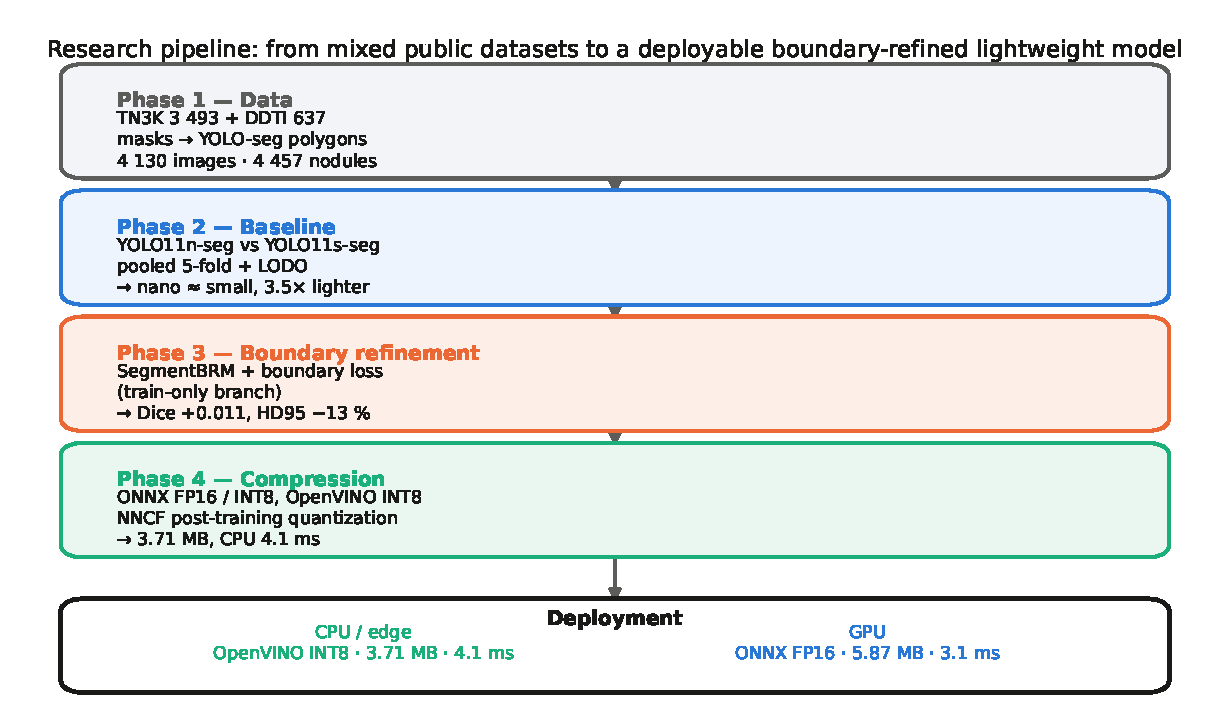
\includegraphics[width=0.92\linewidth]{fig8_pipeline}
  \caption[연구 파이프라인.]{연구 파이프라인. 데이터 정비부터 배포 형식 선택까지의 네 단계와 각 단계의 핵심 결과.}
  \label{fig:pipeline}
\end{figure}

\section{기반 모델: YOLOv11-seg}\label{sec:base_model}

기반 모델은 YOLOv11n-seg\citep{jocher2024yolo11}이다. 640$\times$640 입력에 대해 백본(0--10층,
1,365,472개 파라미터)이 C3k2·SPPF·C2PSA 블록으로 특징을 추출하고, 넥(11--22층, 793,696개)이
FPN·PAN 구조로 스트라이드 8, 16, 32의 세 특징 맵 $\{F_3, F_4, F_5\}$를 만든다. 세 특징 맵의 격자 수를
합한 8,400개 위치가 각각 하나의 예측 후보가 된다.

분할 헤드는 YOLACT\citep{bolya2019yolact}의 프로토타입 방식을 따르며 세 경로로 이루어진다.

\begin{itemize}
  \item \textbf{검출 경로}: 각 위치에서 상자를 DFL\citep{li2020gfl} 분포로 회귀하고 클래스 점수를 예측한다.
  \item \textbf{계수 경로}(\texttt{cv4}): 각 위치에서 길이 $K=32$의 마스크 계수 벡터 $\bm{c}\in\mathbb{R}^{K}$를 예측한다.
    스케일마다 3$\times$3 합성곱 두 개와 1$\times$1 합성곱 하나로 구성된다.
  \item \textbf{프로토타입 경로}(Proto): 가장 고해상도인 $F_3$(80$\times$80)를 입력받아
    3$\times$3 합성곱, 2배 전치 합성곱, 3$\times$3 합성곱, 1$\times$1 합성곱을 거쳐
    입력의 1/4 해상도(160$\times$160)에서 $K$개의 프로토타입 $\bm{P}\in\mathbb{R}^{K\times 160\times 160}$를 만든다.
\end{itemize}

객체 $i$의 마스크는 계수와 프로토타입의 선형 결합으로 만들어진다.
\begin{equation}
  \hat{\bm{m}}_i = \sigma\!\left(\sum_{k=1}^{K} c_{ik}\,\bm{P}_k\right) \in [0,1]^{160\times160}
  \label{eq:proto}
\end{equation}
여기서 $\sigma$는 시그모이드 함수이다. 추론 시에는 이 마스크를 예측 상자 안으로 잘라 원본 해상도로 키운다.
프로토타입 $\bm{P}$는 한 영상의 모든 객체가 공유하므로, \eqnref{eq:proto}의 마스크 품질은 결국
프로토타입이 경계를 얼마나 잘 표현하느냐에 달려 있다. 제안 방법은 이 공유 프로토타입을 개선 대상으로 삼는다.

\section{경계 정교화 모듈: \BRM}\label{sec:brm}

\figref{fig:architecture}는 제안 모델의 구조이다. \BRM{}은 기존 분할 헤드를 대체하지 않고 확장한다.
검출·계수·프로토타입의 세 경로는 그대로 두고, 프로토타입 출력 $\bm{P}$에서 보조 경계 분기 $g_\phi$ 하나를
추가로 갈라낸다.
\begin{equation}
  \hat{\bm{e}} = g_\phi(\bm{P}) = \mathrm{Conv}_{1\times1}^{16\rightarrow1}\Big(\mathrm{SiLU}\big(\mathrm{BN}(\mathrm{Conv}_{3\times3}^{32\rightarrow16}(\bm{P}))\big)\Big)
  \in \mathbb{R}^{1\times160\times160}
  \label{eq:edge_branch}
\end{equation}
$\hat{\bm{e}}$는 각 픽셀이 결절 경계에 속할 로짓이다. 분기의 파라미터는 3$\times$3 합성곱 4,608개, 배치 정규화
32개, 1$\times$1 합성곱 17개로 모두 4,657개이며, 전체 모델(2,847,460개)의 0.16\%이다.

이 분기를 프로토타입 뒤에 둔 이유는 다음과 같다. 경계 분기가 계산하는 손실의 기울기는 $g_\phi$를 거쳐
$\bm{P}$로, 다시 프로토타입 경로와 넥, 백본으로 전파된다. 즉 경계 감독 신호가 모든 객체 마스크가 공유하는
프로토타입에 직접 작용하여, 프로토타입이 경계 정보를 담도록 유도한다. 분기는 이 유도 역할만 하고
마스크 생성에는 관여하지 않으므로, 학습이 끝나면 제거해도 \eqnref{eq:proto}의 결과는 달라지지 않는다.

\begin{figure}[htbp]
  \centering
  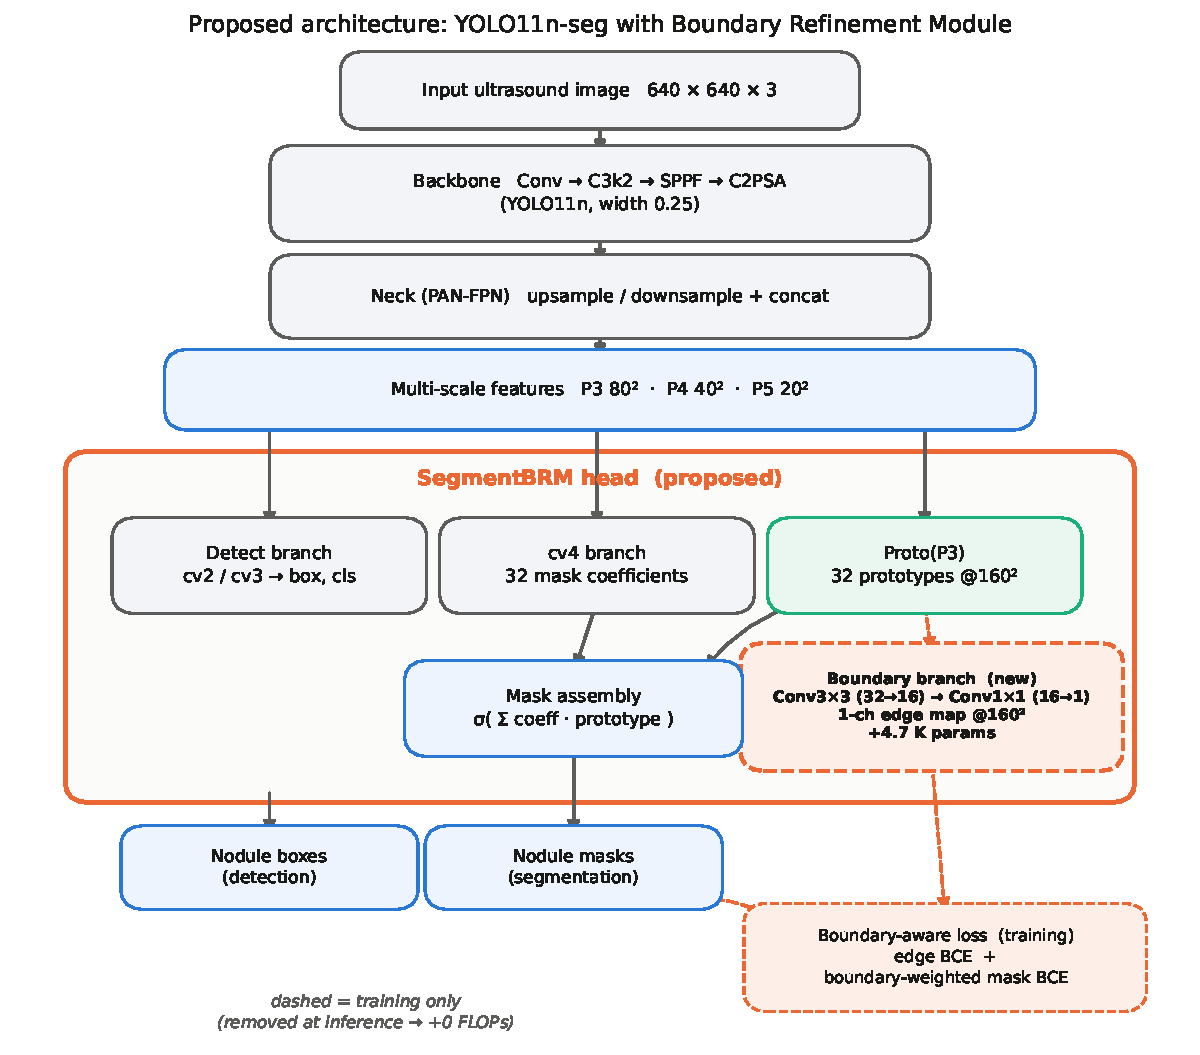
\includegraphics[width=0.85\linewidth]{fig5_architecture}
  \caption[제안 모델의 구조.]{제안 모델의 구조. 점선으로 표시한 경계 분기와 경계 인식 손실은 학습 때만 사용되며,
    추론 그래프에는 포함되지 않는다.}
  \label{fig:architecture}
\end{figure}

\section{경계 인식 손실}\label{sec:boundary_loss}

\subsection{형태학적 경계 밴드}

이진 마스크 $\bm{M}$의 경계 밴드를 형태학적 기울기로 정의한다.
\begin{equation}
  \mathcal{B}(\bm{M}) = \mathrm{clip}\big(\dil_{3\times3}(\bm{M}) - \ero_{3\times3}(\bm{M}),\ 0,\ 1\big)
  \label{eq:band}
\end{equation}
팽창과 침식은 각각 3$\times$3 최대 풀링과 부호를 바꾼 최대 풀링으로 구현하므로, 학습 파라미터가 없고
GPU에서 추가 비용이 거의 없다. 마스크 해상도(160$\times$160)에서 밴드의 폭은 경계 안팎으로 한 픽셀씩
두 픽셀이며, 이는 640 입력 기준 약 8픽셀에 해당한다. \figref{fig:boundary_loss}는 실제 정답 마스크에서
계산한 밴드와 가중치 맵이다.

\begin{figure}[htbp]
  \centering
  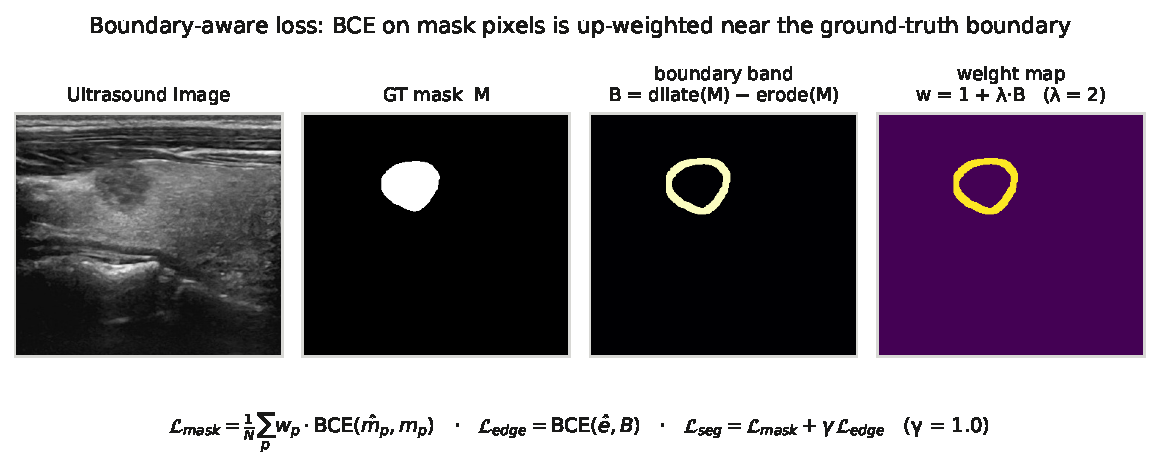
\includegraphics[width=\linewidth]{fig7_boundary_loss}
  \caption[경계 인식 손실의 구성.]{경계 인식 손실의 구성. 초음파 영상, 정답 마스크 $\bm{M}$, 형태학적 경계 밴드 $\mathcal{B}(\bm{M})$,
    가중치 맵 $\bm{w} = 1 + \lambda\mathcal{B}$ ($\lambda=2$).}
  \label{fig:boundary_loss}
\end{figure}

\subsection{경계 가중 마스크 손실}

YOLOv11-seg의 마스크 손실은 양성으로 할당된 각 예측 $j$에 대해, 대응하는 정답 상자 영역 $R_j$ 안의 픽셀별
이진 교차 엔트로피를 평균한다. 제안 손실은 여기에 경계 가중치를 곱한다.
\begin{gather}
  w_p = 1 + \lambda\,\mathcal{B}(\bm{m}_j)_p \label{eq:weight}\\
  \mathcal{L}_{\text{mask}}^{\text{BW}} = \frac{1}{N_{\text{fg}}}\sum_{j=1}^{N_{\text{fg}}} \frac{1}{|R_j|}
    \sum_{p\in R_j} w_p\,\BCE\!\big(\bm{c}_j^{\top}\bm{P}_{:,p},\ m_{jp}\big)
  \label{eq:mask_bw}
\end{gather}
$\bm{m}_j$는 예측 $j$에 할당된 정답 결절의 마스크, $N_{\text{fg}}$는 양성 예측 수이다.
$\lambda=0$이면 원래의 마스크 손실과 같다. $\lambda>0$이면 경계 밴드 픽셀의 오차가 내부 픽셀보다
$(1+\lambda)$배 크게 반영되어, 학습 신호가 경계에 집중된다.

\subsection{보조 경계 손실}

경계 분기의 출력 $\hat{\bm{e}}$는 영상 전체 결절의 합집합 마스크 $\bm{S}$의 경계 밴드를 정답으로 학습한다.
\begin{equation}
  \mathcal{L}_{\text{edge}} = \frac{1}{N_b H W}\sum_{b=1}^{N_b}\sum_{p} \BCE\!\big(\hat{e}_{bp},\ \mathcal{B}(\bm{S}_b)_p\big)
  \label{eq:edge_loss}
\end{equation}
$N_b$는 배치 크기, $H\times W = 160\times160$이다. 정답 마스크는 데이터 로더가 제공하는 인스턴스 마스크를
마스크 해상도로 최근접 보간한 뒤 0보다 큰 픽셀을 전경으로 하여 만든다.

\subsection{전체 손실}

전체 손실은 YOLOv11-seg의 손실 구성에 두 경계 항을 더한 것이다.
\begin{equation}
  \mathcal{L} = N_b\Big[\,\lambda_{\text{box}}\mathcal{L}_{\text{box}} + \lambda_{\text{cls}}\mathcal{L}_{\text{cls}}
  + \lambda_{\text{dfl}}\mathcal{L}_{\text{dfl}}
  + \lambda_{\text{box}}\big(\mathcal{L}_{\text{mask}}^{\text{BW}} + g\,\mathcal{L}_{\text{edge}}\big)\Big]
  \label{eq:total_loss}
\end{equation}
$\mathcal{L}_{\text{box}}$는 CIoU 손실, $\mathcal{L}_{\text{cls}}$는 분류 BCE, $\mathcal{L}_{\text{dfl}}$는
분포 초점 손실이며, 가중치는 YOLOv11 기본값 $\lambda_{\text{box}}=7.5$, $\lambda_{\text{cls}}=0.5$,
$\lambda_{\text{dfl}}=1.5$를 그대로 사용하였다. Ultralytics 구현은 마스크 손실에 상자 손실과 같은 가중치
$\lambda_{\text{box}}$를 쓰므로, 경계 항도 같은 가중치를 공유하도록 하여 원래 손실들과 크기 균형을 맞췄다.
경계 항의 두 계수, 즉 보조 손실 가중치 $g$와 경계 강조 계수 $\lambda$는 \secref{sec:sweep}의 스윕으로
$g=1.0$, $\lambda=2.0$으로 정하였다. 두 경계 항은 학습 로그에서 분할 손실 항목에 합산되므로,
4개 항목으로 이루어진 기존 손실 기록 형식은 바뀌지 않는다. \algref{alg:train_step}은 학습 한 단계의 절차이다.

\begin{algorithm}[htbp]
\caption{\BRM{} 학습 한 단계}\label{alg:train_step}
\begin{algorithmic}[1]
\Require 배치 영상 $\bm{X}$, 정답 상자·클래스, 인스턴스 마스크; 계수 $g$, $\lambda$
\State $\{F_3,F_4,F_5\} \gets \mathrm{Neck}(\mathrm{Backbone}(\bm{X}))$
\State 상자·클래스 예측, 마스크 계수 $\bm{c}$ $\gets$ 검출 경로, 계수 경로$(F_3,F_4,F_5)$
\State $\bm{P} \gets \mathrm{Proto}(F_3)$; \quad $\hat{\bm{e}} \gets g_\phi(\bm{P})$ \Comment{학습 모드에서만 계산}
\State 과제 정렬 할당기로 양성 예측과 정답 결절을 짝짓는다
\State $\mathcal{L}_{\text{box}}, \mathcal{L}_{\text{cls}}, \mathcal{L}_{\text{dfl}}$ 계산
\For{각 양성 예측 $j$}
  \State $\bm{w} \gets 1 + \lambda\,\mathcal{B}(\bm{m}_j)$ \Comment{\eqnref{eq:band}, \eqnref{eq:weight}}
  \State 상자 $R_j$ 안에서 $\bm{w}\odot\BCE(\bm{c}_j^{\top}\bm{P},\ \bm{m}_j)$의 평균을 누적
\EndFor
\State $\mathcal{L}_{\text{edge}} \gets \BCE(\hat{\bm{e}},\ \mathcal{B}(\bm{S}))$ \Comment{\eqnref{eq:edge_loss}}
\State \eqnref{eq:total_loss}로 $\mathcal{L}$을 구하고 역전파하여 모든 파라미터를 갱신
\end{algorithmic}
\end{algorithm}

\section{학습--추론 분리와 추론 비용}\label{sec:dualpath}

\figref{fig:dual_path}는 같은 모델이 학습과 추론에서 서로 다른 경로로 동작하는 모습이다.
학습 모드에서 \BRM{}은 (검출 출력, 마스크 계수, 프로토타입, 경계 로짓)의 네 값을 반환하고, 손실 함수는
네 번째 값이 있을 때만 경계 항을 계산한다. 추론 모드와 ONNX·OpenVINO 변환 모드에서는 경계 분기
$g_\phi$를 아예 호출하지 않고, 기존 분할 헤드와 똑같은 형태의 출력만 반환한다.

따라서 배포되는 연산 그래프는 베이스라인과 동일하다. 실제로 640$\times$640 입력에서 측정한 추론 연산량은
베이스라인과 제안 모델 모두 9.73 GFLOPs로 같았다(\tabref{tab:brm_main}). 경계 분기의 가중치 4,657개는
PyTorch 체크포인트 파일에만 남아 파일 크기를 6.00 MB에서 6.01 MB로 늘릴 뿐, 변환된 추론 그래프에는
포함되지 않는다. 이 분리 덕분에 경계 품질 향상이 추론 비용 증가라는 대가를 요구하지 않는다.

\begin{figure}[htbp]
  \centering
  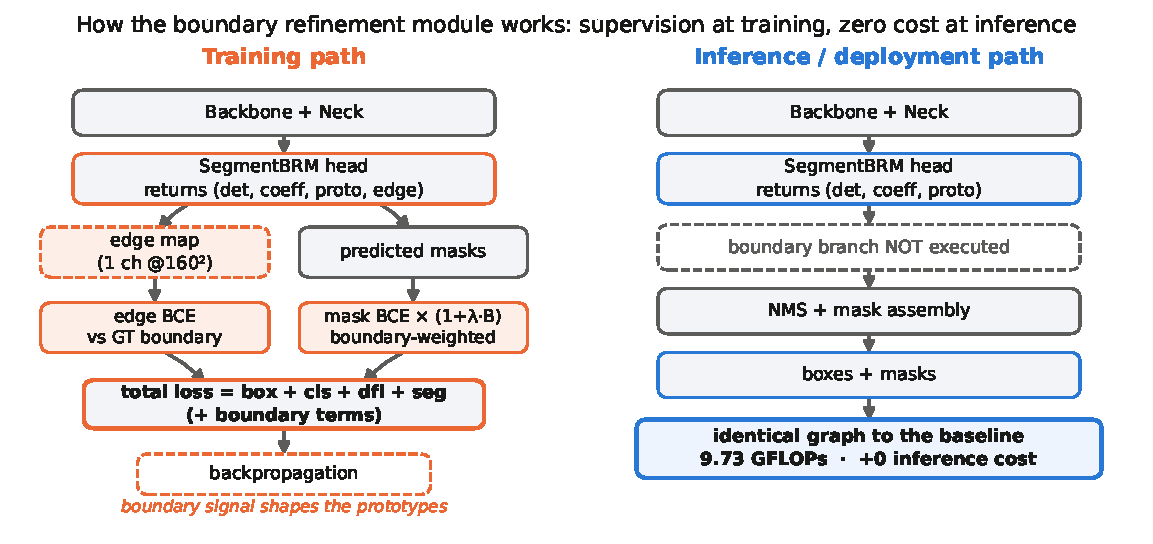
\includegraphics[width=\linewidth]{fig6_dual_path}
  \caption[학습 경로와 추론 경로.]{학습 경로와 추론 경로. 학습 때는 경계 분기가 프로토타입에 경계 신호를 전달하고,
    추론 때는 분기가 실행되지 않아 베이스라인과 같은 그래프가 된다.}
  \label{fig:dual_path}
\end{figure}

\section{사후 양자화 파이프라인}\label{sec:quant}

제안 모델을 재학습 없이 배포 형식으로 바꾸기 위해 다섯 가지 정밀도를 준비하였다.

\paragraph{ONNX FP32 / FP16.} Ultralytics 변환 기능으로 opset 13의 ONNX 그래프를 만들고 그래프 단순화를
적용하였다. FP16은 GPU에서 반정밀도로 변환하였다.

\paragraph{ONNX Runtime 정적 INT8.} ONNX FP32 모델에 전처리(형상 추론·그래프 정리)를 적용한 뒤, ONNX Runtime의
정적 양자화를 QDQ 형식으로 수행하였다. 가중치는 채널별 부호 있는 INT8, 활성값은 부호 없는 INT8이며,
캘리브레이션에는 TN3K 학습·검증 분할에서 무작위로 뽑은 150장(시드 42)을 추론과 같은 방식
(640 레터박스, 0--1 정규화)으로 전처리하여 사용하였다. 채널별 QDQ 양자화는 opset 13 이상에서만 유효한
그래프가 만들어진다.

이 과정에서 중요한 실패를 확인하였다. 그래프 전체를 양자화하면 모든 클래스 점수가 0이 되어 아무것도
검출되지 않는다. 헤드의 시그모이드 직전 로짓과 DFL 분포처럼 출력 단의 작은 값 차이가 결과를 좌우하는
연산이 8비트 해상도로 표현되면서 정보가 손실된 것으로 추정된다. OpenVINO 변환 경로가 바로 이 연산들을
양자화에서 제외하도록 설계되어 있다는 점(아래)도 이 해석을 뒷받침한다. 그래서 분할 헤드(그래프의
\texttt{/model.23/} 이하 119개 노드)를 양자화 대상에서 제외하고 부동소수점으로 남겼으며, 이렇게 하자
검출 출력이 정상으로 돌아왔다.

\paragraph{OpenVINO INT8.} Ultralytics의 OpenVINO 변환 기능으로 FP32 IR을 만든 뒤 NNCF\citep{kozlov2020nncf}로
사후 양자화하였다. 양자화 방식은 NNCF의 MIXED 프리셋(가중치 대칭, 활성값 비대칭)이며, 캘리브레이션에는
해당 fold의 검증 분할 영상을 사용하였다. 이 경로에서는 헤드 전체가 아니라 헤드 안의 덧셈·뺄셈·곱셈·나눗셈
연산, DFL 연산, 그리고 모든 시그모이드 연산만 양자화 범위에서 제외된다. 즉 헤드의 합성곱, 특히 160$\times$160
해상도에서 동작하는 프로토타입 경로의 합성곱은 INT8로 바뀐다. 두 INT8 경로의 지연 시간 차이는 대부분
이 제외 범위의 차이에서 비롯된다(\secref{sec:disc_quant}).

\paragraph{배포 형식 선택.} 정확도는 모든 정밀도에서 같은 held-out 집합과 같은 평가 코드로 다시 측정하였다.
INT8 모델은 배포 대상인 CPU에서, FP32·FP16 모델은 GPU에서 평가하였다.

% ============================================================================
\chapter{실험 및 결과}\label{ch:experiments}
% ============================================================================

이 장은 실험 환경과 평가 방법(\secref{sec:exp_env}--\secref{sec:exp_eval})을 먼저 설명한 뒤, 결과를 가설 순서에
따라 제시한다. H1은 \secref{sec:exp_baseline}, H2는 \secref{sec:sweep}--\secref{sec:exp_lodo},
H3은 \secref{sec:exp_quant}에서 다루고, \secref{sec:exp_final}에서 단계별 누적 결과를 정리한다.

\section{실험 환경}\label{sec:exp_env}

\tabref{tab:env}는 실험에 사용한 하드웨어와 소프트웨어이다. 학습과 GPU 지연 측정은 NVIDIA A100 GPU에서,
CPU 지연 측정은 같은 서버의 CPU에서 수행하였다.

% 자동 생성 파일 — scripts/make_thesis.py 가 덮어쓴다. 직접 고치지 말 것.
\begin{table}[htbp]
\centering
\small
\caption{실험 환경.}
\label{tab:env}
\begin{adjustbox}{max width=\linewidth}
\begin{tabular}{ll}
\toprule
항목 & 사양 \\
\midrule
GPU & NVIDIA A100-SXM4-80GB, 81920 MiB $\times$ 3 \\
CPU & AMD EPYC 9654 96-Core Processor (192 논리 코어) \\
Python / PyTorch / CUDA & 3.10.18 / 2.5.1+cu121 / 12.1 \\
Ultralytics & 8.3.181 (커스텀 패치 적용) \\
ONNX Runtime & 1.23.0 \\
OpenVINO / NNCF & 2026.2.1 / 3.2.0 \\
NumPy / SciPy / OpenCV & 2.1.2 / 1.15.3 / 4.12.0 \\
\bottomrule
\end{tabular}
\end{adjustbox}
\end{table}


\section{학습 설정}\label{sec:exp_train}

모든 모델은 COCO 사전학습 가중치(\texttt{yolo11n-seg.pt}, \texttt{yolo11s-seg.pt})에서 미세 조정하였다.
제안 모델은 제안 구성 파일로 모델을 만든 뒤 같은 사전학습 가중치를 이식하였으며, 새로 추가된 경계 분기만
무작위로 초기화된다. 학습 설정은 \tabref{tab:hparams}와 같다. 옵티마이저는 Ultralytics의 자동 선택에 맡겼으며,
전체 반복 횟수에 따라 AdamW(학습률 0.002, 모멘텀 0.9)가 선택되었다. 최대 100 epoch 동안 학습하되 검증 fitness가
20 epoch 동안 개선되지 않으면 조기 종료하였고, 검증 fitness가 가장 높은 epoch의 가중치를 최종 모델로 사용하였다.
fold별 실제 학습 epoch은 \tabref{tab:epochs}에 있다.

% 자동 생성 파일 — scripts/make_thesis.py 가 덮어쓴다. 직접 고치지 말 것.
\begin{table}[htbp]
\centering
\small
\caption[학습 설정.]{학습 설정. 베이스라인과 제안 모델은 경계 손실 계수를 제외한 모든 값이 같다(생성 시 두 모델의 \texttt{args.yaml}이 일치하는지 자동 확인함).}
\label{tab:hparams}
\begin{adjustbox}{max width=\linewidth}
\begin{tabular}{lp{0.74\linewidth}}
\toprule
구분 & 설정값 \\
\midrule
최적화 & \parbox[t]{0.72\linewidth}{\raggedright \texttt{epochs}=100, \texttt{patience}=20, \texttt{batch}=32, \texttt{imgsz}=640, \texttt{optimizer}=auto, \texttt{lr0}=0.01, \texttt{lrf}=0.01, \texttt{momentum}=0.937, \texttt{weight\_decay}=0.0005, \texttt{warmup\_epochs}=3.0, \texttt{cos\_lr}=False, \texttt{amp}=True} \\
손실 가중치 & \parbox[t]{0.72\linewidth}{\raggedright \texttt{box}=7.5, \texttt{cls}=0.5, \texttt{dfl}=1.5, \texttt{overlap\_mask}=True, \texttt{mask\_ratio}=4} \\
데이터 증강 & \parbox[t]{0.72\linewidth}{\raggedright \texttt{hsv\_h}=0.015, \texttt{hsv\_s}=0.7, \texttt{hsv\_v}=0.4, \texttt{degrees}=0.0, \texttt{translate}=0.1, \texttt{scale}=0.5, \texttt{shear}=0.0, \texttt{perspective}=0.0, \texttt{flipud}=0.0, \texttt{fliplr}=0.5, \texttt{mosaic}=1.0, \texttt{close\_mosaic}=10, \texttt{mixup}=0.0, \texttt{copy\_paste}=0.0} \\
재현성 & \parbox[t]{0.72\linewidth}{\raggedright \texttt{seed}=42, \texttt{deterministic}=True} \\
경계 손실 (제안) & \texttt{head\_gain}=1.0, $\lambda$=2.0 (\ref{sec:sweep}절 스윕으로 결정) \\
\bottomrule
\end{tabular}
\end{adjustbox}
\end{table}


\section{평가 방법}\label{sec:exp_eval}

\subsection{정확도 지표}

\paragraph{Mask \mAP{}.} Ultralytics의 검증 절차로 held-out 집합에서 계산한 마스크 기준 평균 정밀도로,
IoU 임계값 0.50부터 0.95까지 0.05 간격의 10개 임계값에 대한 평균이다.

\paragraph{경계 지표.} 경계 지표는 의미 분할 형태로 계산한다. 신뢰도 0.25 이상, NMS IoU 0.7로 얻은 예측
결절들을 원본 해상도 마스크로 복원하여 합집합 $\bm{P}$를 만들고, 정답 결절 다각형의 합집합 $\bm{G}$와 비교한다.
영상 $I$의 높이·너비를 $h, w$, 대각선 길이를 $D=\sqrt{h^2+w^2}$라 하자.

\begin{itemize}
  \item \textbf{Dice}: $\mathrm{Dice} = 2|\bm{G}\cap\bm{P}| / (|\bm{G}|+|\bm{P}|)$. 두 마스크가 모두 비어 있으면 1로 둔다.
  \item \textbf{HD95}: 마스크와 그 1픽셀 침식의 차로 경계 $\partial\bm{G}, \partial\bm{P}$를 얻고, 거리 변환으로
    한 경계의 각 점에서 다른 경계까지의 거리 $d(\cdot,\cdot)$를 구한다.
    \begin{equation}
      \mathrm{HD95} = \frac{100}{D}\max\Big\{\, P_{95}\big(d(x,\partial\bm{P})\big)_{x\in\partial\bm{G}},\
      P_{95}\big(d(y,\partial\bm{G})\big)_{y\in\partial\bm{P}} \Big\}
      \label{eq:hd95}
    \end{equation}
    $P_{95}$는 95 백분위값이다. 해상도가 영상마다 다르므로 대각선 대비 백분율로 정규화하였다. 예측이나 정답 중
    한쪽의 경계가 없으면 최대 벌점 100\%를 준다.
  \item \textbf{Boundary IoU}\citep{cheng2021boundaryiou}: 폭 $d=\mathrm{round}(0.02D)$의 경계 띠
    $\bm{G}_d = \bm{G} - \ero_d(\bm{G})$, $\bm{P}_d = \bm{P} - \ero_d(\bm{P})$에서 IoU를 구한다.
    \begin{equation}
      \mathrm{BIoU} = \frac{|\bm{G}_d\cap\bm{P}_d|}{|\bm{G}_d\cup\bm{P}_d|}
      \label{eq:biou}
    \end{equation}
    $\ero_d$는 반지름 $d$인 타원형 구조 요소로 침식하는 연산이다.
\end{itemize}

세 경계 지표는 영상마다 계산한 뒤 평균한다. 따라서 결절이 큰 영상이 평균을 지배하지 않는다.

\subsection{효율 지표}

파라미터 수와 640$\times$640 입력 기준 GFLOPs를 보고하고, 지연 시간은 전처리와 후처리(NMS 등)를 제외한
순수 순전파 시간으로 측정하였다. batch 1의 640$\times$640 입력으로 15회 워밍업한 뒤 100회 반복 실행한 평균이다.
ONNX 모델은 ONNX Runtime의 CPU·CUDA 실행 공급자로, OpenVINO 모델은 OpenVINO 런타임의 CPU 장치로 측정하였다.

\subsection{통계 검정}\label{sec:exp_stats}

평균의 차이가 우연의 범위 안인지를 판단하기 위해 세 단위에서 대응표본 검정을 수행하였다.

\begin{itemize}
  \item \textbf{영상 단위 (주 분석).} held-out 614장 각각에 대해, 5개 fold 모델의 지표를 평균한 값을 베이스라인과
    제안 모델 사이에서 짝지어 비교한다. Wilcoxon 부호 순위 검정\citep{wilcoxon1945}(양측)과 대응 $t$ 검정을 함께
    보고하고, 평균 차이의 95\% 신뢰구간을 10,000회 부트스트랩\citep{efron1993bootstrap} 백분위 구간으로 구한다.
  \item \textbf{fold 단위 (보조).} 5개 fold의 평균 지표를 짝지어 비교한다. 학습의 무작위성까지 오차로 포함하는
    보수적인 분석이지만 표본이 5개뿐이어서 검정력이 매우 낮다.
  \item \textbf{시드 단위 (교차 데이터셋).} LODO 실험은 시드 3개(42, 43, 44)의 평균 지표를 대응 $t$ 검정으로 비교한다.
\end{itemize}

효과크기는 대응표본 Cohen's $d_z$\citep{lakens2013effect}, 즉 대응 차이의 평균을 그 표준편차로 나눈 값으로 보고한다.
HD95는 작을수록 좋으므로 부호를 바꾸어, 모든 지표에서 양수가 제안 모델의 우세를 뜻하도록 통일하였다.
'개선 비율'은 대응 차이가 제안 모델 쪽으로 나온 표본의 비율이다.

영상 단위 분석은 테스트 영상의 표본 변동을 오차로 삼으므로 "이 학습 절차로 얻은 모델들이 새 영상에서 더 나은가"에
답한다. 반면 학습 자체의 무작위성은 fold·시드 단위 분석이 반영한다. 두 단위의 결과를 함께 보고하는 이유가
여기에 있으며, 그 해석은 \secref{sec:disc_lodo}에서 다시 다룬다.

\section{기준 모델 선정 (H1)}\label{sec:exp_baseline}

\tabref{tab:nano_small}은 nano와 small을 같은 조건에서 학습하여 held-out 집합에서 비교한 결과이다.

% 자동 생성 파일 — scripts/make_thesis.py 가 덮어쓴다. 직접 고치지 말 것.
\begin{table}[htbp]
\centering
\small
\caption[YOLOv11-seg nano와 small의 비교 (held-out TN3K test, 5-fold 평균 $\pm$ 표준편차).]{YOLOv11-seg nano와 small의 비교 (held-out TN3K test, 5-fold 평균 $\pm$ 표준편차). 굵은 글씨는 더 나은 값이다.}
\label{tab:nano_small}
\begin{adjustbox}{max width=\linewidth}
\begin{tabular}{lcc}
\toprule
지표 & YOLOv11n-seg (nano) & YOLOv11s-seg (small) \\
\midrule
Mask mAP$_{50:95}$ & \textbf{0.6272 $\pm$ 0.0075} & 0.6239 $\pm$ 0.0084 \\
Mask mAP$_{50}$ & \textbf{0.9071 $\pm$ 0.0057} & 0.9067 $\pm$ 0.0073 \\
Box mAP$_{50:95}$ & \textbf{0.6216 $\pm$ 0.0126} & 0.6181 $\pm$ 0.0121 \\
Box mAP$_{50}$ & \textbf{0.9098 $\pm$ 0.0064} & 0.9080 $\pm$ 0.0090 \\
Mask 정밀도 & 0.8757 $\pm$ 0.0182 & \textbf{0.8784 $\pm$ 0.0261} \\
Mask 재현율 & 0.8300 $\pm$ 0.0085 & \textbf{0.8431 $\pm$ 0.0201} \\
\midrule
파라미터 & \textbf{2.84 M} & 10.08 M (3.5배) \\
GFLOPs & \textbf{9.73} & 33.08 (3.4배) \\
가중치 파일 크기 & \textbf{6.00 MB} & 20.51 MB (3.4배) \\
\bottomrule
\end{tabular}
\end{adjustbox}
\end{table}


nano는 Mask \mAP{} 0.6272로 small(0.6239)보다 오히려 근소하게 높았고, Box \mAP{}에서도 0.6216 대 0.6181로
앞섰다. 두 모델의 차이는 모두 fold 표준편차(약 0.008)보다 작아 사실상 같은 수준이다. small은 Mask 재현율이
0.8431로 nano(0.8300)보다 0.013 높았지만 이 역시 small의 fold 표준편차(0.020) 안에 있다. 반면 small은 파라미터
3.5배, 연산량 3.4배, 파일 크기 3.4배를 더 쓴다. 단일 클래스이고 형태 변이가 제한적인 결절 분할에서는 small의
추가 용량이 정확도로 이어지지 않은 것이다. 따라서 \textbf{H1은 지지되며}, 이후 모든 실험은 nano를 기준 모델로 한다.

\section{경계 손실 계수 탐색}\label{sec:sweep}

경계 인식 손실에는 보조 경계 손실 가중치 $g$와 경계 밴드 강조 계수 $\lambda$의 두 계수가 있다
(\eqnref{eq:total_loss}). 처음에는 $g=0.5$, $\lambda=5$로 5개 fold 전체를 학습하였으나, 경계 지표의 개선이 fold마다
엇갈리고 Mask \mAP{}가 0.627에서 0.621로 떨어졌다. 그래서 $g\in\{0.25, 1.0\}$, $\lambda\in\{2, 10\}$의 4개 구성을,
초기값에서 효과의 방향이 갈렸던 fold 0과 2에서 학습하여 비교하였다.

\paragraph{스윕 당시의 선택.} \tabref{tab:sweep_test}는 스윕 모델을 held-out 집합에서 평가한 결과이며, 스윕 당시에는
이 표를 근거로 계수를 골랐다. 다섯 BRM 구성 모두 Dice와 HD95에서 베이스라인보다 나았고, 그중 $g=1.0$, $\lambda=2.0$이
네 지표 모두에서 가장 좋았다. 특히 이 구성만 Mask \mAP{}를 베이스라인 이상(0.6338 대 0.6306)으로 유지하였고,
나머지 구성은 0.010 안팎 낮았다. 이에 따라 $g=1.0$, $\lambda=2.0$을 채택하였다.

% 자동 생성 파일 — scripts/make_thesis.py 가 덮어쓴다. 직접 고치지 말 것.
\begin{table}[htbp]
\centering
\small
\caption[경계 손실 계수 탐색 결과 (fold 0·2 평균, held-out TN3K test 614장).]{경계 손실 계수 탐색 결과 (fold 0·2 평균, held-out TN3K test 614장). $g$는 보조 경계 손실 가중치(\texttt{head\_gain}), $\lambda$는 경계 밴드 강조 계수이며, 굵은 글씨가 채택한 구성이다. 스윕 당시 이 표를 근거로 계수를 선택하였다(\secref{sec:sweep}의 한계 참조).}
\label{tab:sweep_test}
\begin{adjustbox}{max width=\linewidth}
\begin{tabular}{lcccccc}
\toprule
구분 & $g$ & $\lambda$ & Dice$\uparrow$ & HD95 (\%)$\downarrow$ & BIoU$\uparrow$ & Mask mAP$_{50:95}\uparrow$ \\
\midrule
베이스라인 & -- & -- & 0.8132 & 10.835 & 0.4357 & 0.6306 \\
\midrule
초기값 & 0.5 & 5 & 0.8243 & 8.759 (-19.2\%) & 0.4348 & 0.6209 \\
\midrule
스윕 & 0.25 & 2 & 0.8301 & 8.565 (-21.0\%) & 0.4372 & 0.6199 \\
스윕 & 0.25 & 10 & 0.8264 & 8.607 (-20.6\%) & 0.4377 & 0.6203 \\
\textbf{스윕} & \textbf{1} & \textbf{2} & \textbf{0.8368} & \textbf{7.995 (-26.2\%)} & \textbf{0.4473} & \textbf{0.6338} \\
스윕 & 1 & 10 & 0.8258 & 8.378 (-22.7\%) & 0.4318 & 0.6192 \\
\bottomrule
\end{tabular}
\end{adjustbox}
\end{table}


\paragraph{검증 분할을 이용한 사후 점검.} 그러나 평가 집합으로 하이퍼파라미터를 고르면, 선택된 구성의 평가 성능은
선택 과정 자체 때문에 낙관적으로 편향될 수 있다. 이 문제를 확인하기 위해 같은 스윕 모델들을 각 fold의 검증 분할
(학습에 쓰이지 않고 조기 종료에만 쓰인 영상)에서 다시 평가하였다(\tabref{tab:sweep_val}).

% 자동 생성 파일 — scripts/make_thesis.py 가 덮어쓴다. 직접 고치지 말 것.
\begin{table}[htbp]
\centering
\small
\caption[경계 손실 계수 탐색 결과 (fold 0·2 평균, 각 fold의 검증 분할(fold 0: 704장, fold 2: 703장)).]{경계 손실 계수 탐색 결과 (fold 0·2 평균, 각 fold의 검증 분할(fold 0: 704장, fold 2: 703장)). $g$는 보조 경계 손실 가중치(\texttt{head\_gain}), $\lambda$는 경계 밴드 강조 계수이며, 굵은 글씨가 채택한 구성이다. 계수 선택 이후에 같은 모델을 다시 평가한 사후 점검 결과이다.}
\label{tab:sweep_val}
\begin{adjustbox}{max width=\linewidth}
\begin{tabular}{lcccccc}
\toprule
구분 & $g$ & $\lambda$ & Dice$\uparrow$ & HD95 (\%)$\downarrow$ & BIoU$\uparrow$ & Mask mAP$_{50:95}\uparrow$ \\
\midrule
베이스라인 & -- & -- & 0.7954 & 10.574 & 0.3714 & 0.5617 \\
\midrule
초기값 & 0.5 & 5 & 0.8085 & 8.707 (-17.7\%) & 0.3789 & 0.5660 \\
\midrule
스윕 & 0.25 & 2 & 0.8088 & 8.567 (-19.0\%) & 0.3786 & 0.5612 \\
스윕 & 0.25 & 10 & 0.8052 & 9.068 (-14.2\%) & 0.3805 & 0.5649 \\
\textbf{스윕} & \textbf{1} & \textbf{2} & \textbf{0.8041} & \textbf{9.066 (-14.3\%)} & \textbf{0.3798} & \textbf{0.5635} \\
스윕 & 1 & 10 & 0.8057 & 9.137 (-13.6\%) & 0.3769 & 0.5599 \\
\bottomrule
\end{tabular}
\end{adjustbox}
\end{table}


결과는 두 가지로 요약된다. 첫째, \textbf{경계 정교화의 효과 자체는 선택 절차와 무관하게 재현되었다.} 검증 분할에서도
다섯 BRM 구성 모두 베이스라인보다 Dice가 0.009--0.013 높고, HD95가 13.6--19.0\% 낮고, Boundary IoU가 0.006--0.009 높았다.
Mask \mAP{}는 베이스라인과 $\pm$0.005 이내였다. 둘째, \textbf{구성 사이의 순위는 재현되지 않았다.} held-out에서 모든 지표
1위였던 $g=1.0$, $\lambda=2.0$은 검증 분할에서 Dice가 BRM 구성 가운데 가장 낮았고 HD95는 세 번째였으며, 검증 분할에서는
$g=0.25$, $\lambda=2.0$이 Dice와 HD95 모두 가장 좋았다. 다만 검증 분할에서 구성 간 차이(Dice 0.0047, HD95 0.57\%p)는
BRM과 베이스라인의 차이보다 훨씬 작다.

두 결과를 종합하면, $g$와 $\lambda$를 이 범위 안에서 어떻게 고르든 경계 정교화의 이득은 나타나지만, 채택한 구성이
다른 구성보다 특별히 낫다는 근거는 held-out 결과에만 있다. 따라서 \secref{sec:exp_brm}의 최종 개선 폭은 계수 선택 과정의
영향을 받아 실제보다 클 수 있으며, 그 크기는 현재 실험으로 정할 수 없다(\secref{sec:limitations}).
한편 $\lambda=2$가 $\lambda=10$보다 HD95에서 나은 경향은 두 $g$ 값과 두 평가 집합 네 경우 모두에서 일관되었다.
이 현상의 원인은 \secref{sec:disc_lambda}에서 논의한다.

\section{경계 정교화 결과 (H2)}\label{sec:exp_brm}

채택한 계수($g=1.0$, $\lambda=2.0$)로 제안 모델을 5개 fold 전부에서 처음부터 다시 학습하여 베이스라인과 비교하였다
(\tabref{tab:brm_main}, \figref{fig:boundary_improvement}).

% 자동 생성 파일 — scripts/make_thesis.py 가 덮어쓴다. 직접 고치지 말 것.
\begin{table}[htbp]
\centering
\small
\caption[경계 정교화 모듈의 효과 (held-out TN3K test 614장, 5-fold 평균 $\pm$ 표준편차).]{경계 정교화 모듈의 효과 (held-out TN3K test 614장, 5-fold 평균 $\pm$ 표준편차). 마지막 열은 제안 모델이 베이스라인보다 나은 fold 수이다.}
\label{tab:brm_main}
\begin{adjustbox}{max width=\linewidth}
\begin{tabular}{lcccc}
\toprule
지표 & 베이스라인 & 제안 (BRM) & $\Delta$ (상대) & 개선 fold \\
\midrule
Mask mAP$_{50:95}\uparrow$ & 0.6272 $\pm$ 0.0075 & 0.6267 $\pm$ 0.0081 & -0.0005 (-0.1\%) & 2/5 \\
Dice$\uparrow$ & 0.8195 $\pm$ 0.0070 & 0.8300 $\pm$ 0.0039 & +0.0104 (+1.3\%) & 5/5 \\
HD95 (\%)$\downarrow$ & 9.628 $\pm$ 1.175 & 8.378 $\pm$ 0.775 & -1.249 (-13.0\%) & 3/5 \\
Boundary IoU$\uparrow$ & 0.4358 $\pm$ 0.0072 & 0.4414 $\pm$ 0.0050 & +0.0055 (+1.3\%) & 4/5 \\
\midrule
파라미터 & 2,842,803 & 2,847,460 & +4,657 & -- \\
추론 GFLOPs & 9.73 & 9.73 & +0.00 & -- \\
\bottomrule
\end{tabular}
\end{adjustbox}
\end{table}


\begin{figure}[htbp]
  \centering
  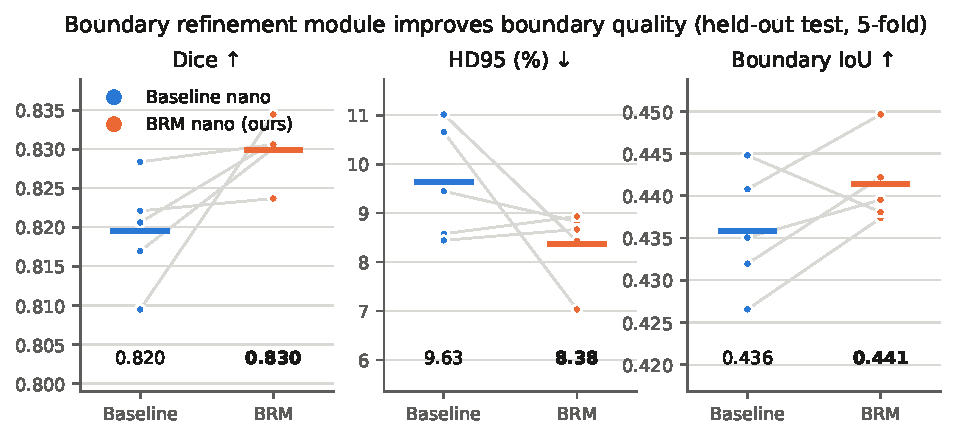
\includegraphics[width=0.92\linewidth]{fig1_boundary_improvement}
  \caption[경계 정교화의 효과 (held-out TN3K test).]{경계 정교화의 효과 (held-out TN3K test). 점은 fold별 값, 회색 선은 같은 fold끼리의 대응,
    가로 막대는 5-fold 평균이다.}
  \label{fig:boundary_improvement}
\end{figure}

세 경계 지표가 모두 개선되었다. Dice는 0.8195에서 0.8300으로 0.0104 올랐고 5개 fold 모두에서 개선되었다.
HD95는 9.628\%에서 8.378\%로 13.0\% 줄었으며, Boundary IoU는 0.4358에서 0.4414로 올랐다(4/5 fold 개선).
fold 간 표준편차도 Dice 0.0070$\rightarrow$0.0039, HD95 1.175$\rightarrow$0.775로 줄어, 제안 모델의 결과가 분할에 덜
민감하였다. HD95는 5개 중 3개 fold에서 개선되었는데, 개선되지 않은 두 fold도 차이가 작았던 반면 개선된 fold의
감소 폭이 커서(\tabref{tab:perfold}) 평균이 크게 줄었다.

Mask \mAP{}는 0.6272에서 0.6267로 사실상 같았다. mAP가 경계 개선을 반영하지 못하는 이유는
\secref{sec:disc_map}에서 논의한다. 추가 파라미터는 4,657개이고 추론 GFLOPs는 9.73으로 같으므로,
경계 개선은 추론 비용 증가 없이 얻은 것이다.

\section{정성적 분석}\label{sec:exp_qual}

\figref{fig:qualitative}는 held-out 영상에서의 예측 경계이다. 개선 폭이 큰 사례만 고르면 그림이 결론을 과장하므로,
무작위로 뽑은 40장 중 결절이 있고 두 모델 모두 예측을 낸 영상을 Dice 개선 폭으로 정렬한 뒤 최상위, 상위 4분위,
중앙값, 최하위에서 한 장씩 골랐다.

\begin{figure}[htbp]
  \centering
  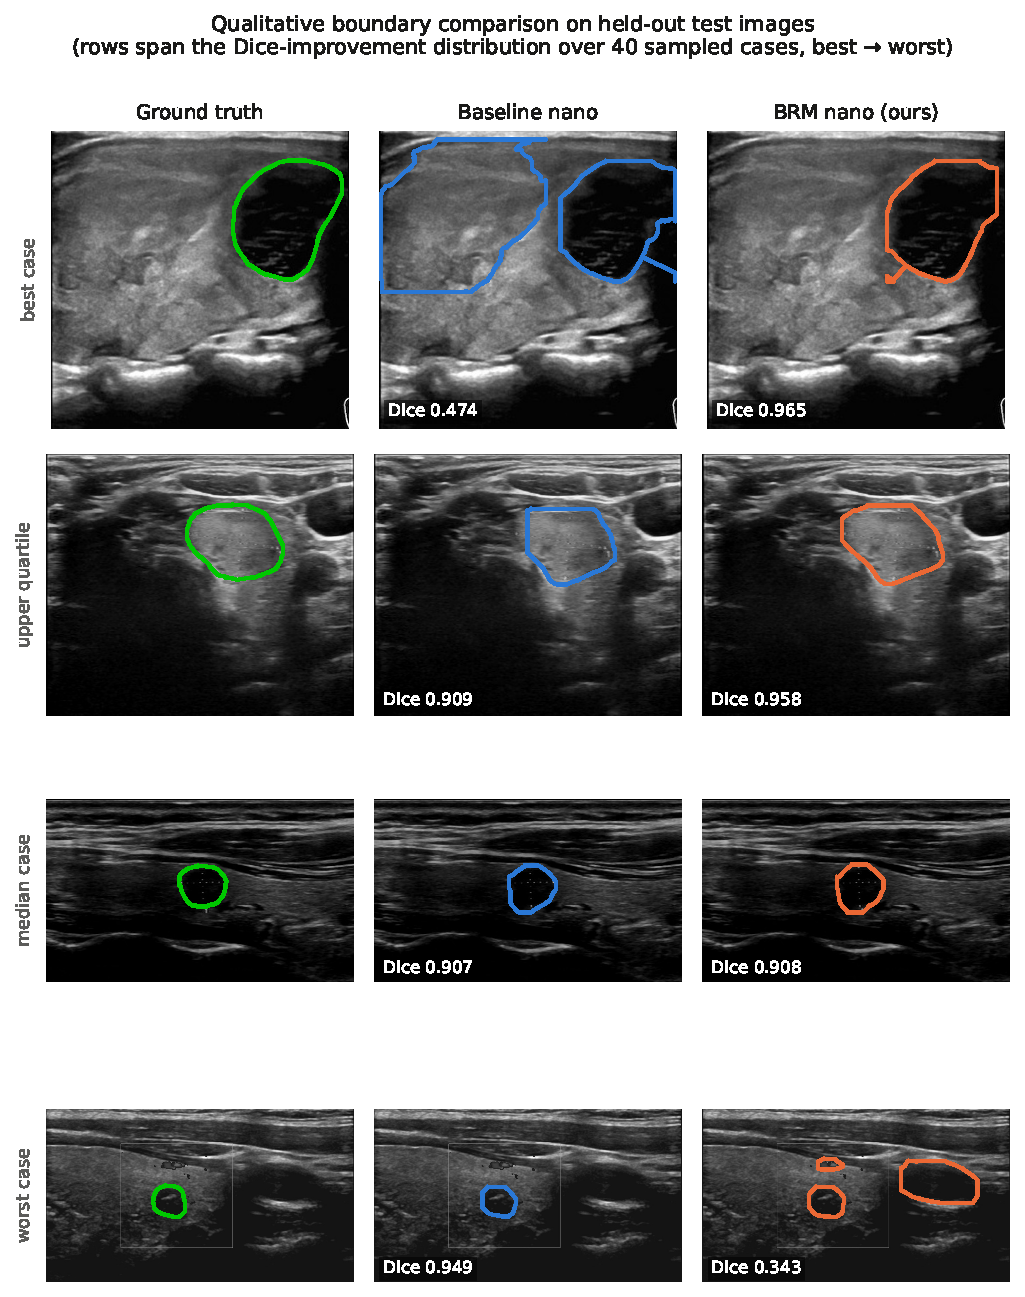
\includegraphics[width=0.72\linewidth]{fig4_qualitative}
  \caption[정성 비교.]{정성 비교. 왼쪽부터 정답 경계, 베이스라인 예측, 제안 모델 예측이며, 행은 위에서부터 Dice 개선 폭의
    최상위·상위 4분위·중앙값·최하위 사례이다. 각 칸의 숫자는 해당 영상의 Dice이다.}
  \label{fig:qualitative}
\end{figure}

상위 사례에서는 제안 모델의 윤곽이 정답에 더 밀착하며, 특히 결절 하방의 음향 음영 구간에서 베이스라인의 경계가
바깥으로 새어 나가는 현상이 줄었다. 중앙값 사례에서는 두 모델의 차이가 거의 없는데, 이는 \secref{sec:exp_sig}의
'개선 비율'이 50\%를 조금 넘는 수준이라는 결과와 일치한다. 최하위 사례는 제안 모델이 결절 옆의 조직을 결절로
함께 포함하여 Dice가 크게 떨어진 경우로, 경계 가중이 잘못 잡힌 경계를 오히려 강화할 수 있음을 보여 주는
실패 유형이다.

\section{통계적 유의성}\label{sec:exp_sig}

\tabref{tab:stats}와 \figref{fig:significance}는 \secref{sec:exp_stats}의 대응표본 검정 결과이다.

% 자동 생성 파일 — scripts/make_thesis.py 가 덮어쓴다. 직접 고치지 말 것.
\begin{table*}[htbp]
\centering
\footnotesize
\caption[경계 정교화 효과의 대응표본 검정 (held-out TN3K test).]{경계 정교화 효과의 대응표본 검정 (held-out TN3K test). 영상 단위 분석은 각 영상에 대해 5개 fold 모델의 예측 지표를 평균한 뒤 비교한다. 95\% 신뢰구간은 대응 차이의 부트스트랩(10,000회) 백분위 구간이며, $d_z$는 대응표본 효과크기로 양수가 제안 모델의 우세를 뜻한다. n=5에서 양측 Wilcoxon 검정이 도달할 수 있는 최소 $p$는 0.0625이다. 대응 $t$ 검정의 $p$는 영상 단위 0.0007, 0.0202, 0.0002, fold 단위 0.071, 0.165, 0.190(Dice, Boundary IoU, HD95 순)로 결론이 같다.}
\label{tab:stats}
\setlength{\tabcolsep}{4pt}
\begin{adjustbox}{max width=\linewidth}
\begin{tabular}{llccccc}
\toprule
분석 단위 & 지표 & $\Delta$ & 95\% CI & Wilcoxon $p$ & $d_z$ & 개선 비율 (\%) \\
\midrule
\multirow{3}{*}{영상 단위 (n=614)} & Dice & +0.0104 & [+0.0044, +0.0166] & $0.014$ (*) & 0.14 & 52.8 \\
 & Boundary IoU & +0.0055 & [+0.0009, +0.0102] & $0.011$ (*) & 0.09 & 53.6 \\
 & HD95 (\%) & -1.2495 & [-1.8945, -0.5918] & $0.0045$ (**) & 0.15 & 53.4 \\
\midrule
\multirow{3}{*}{fold 단위 (n=5)} & Dice & +0.0104 & -- & $0.062$ (n.s.) & 1.09 & 100.0 \\
 & Boundary IoU & +0.0055 & -- & $0.188$ (n.s.) & 0.76 & 80.0 \\
 & HD95 (\%) & -1.2495 & -- & $0.312$ (n.s.) & 0.71 & 60.0 \\
\bottomrule
\end{tabular}
\end{adjustbox}
\end{table*}


\begin{figure}[htbp]
  \centering
  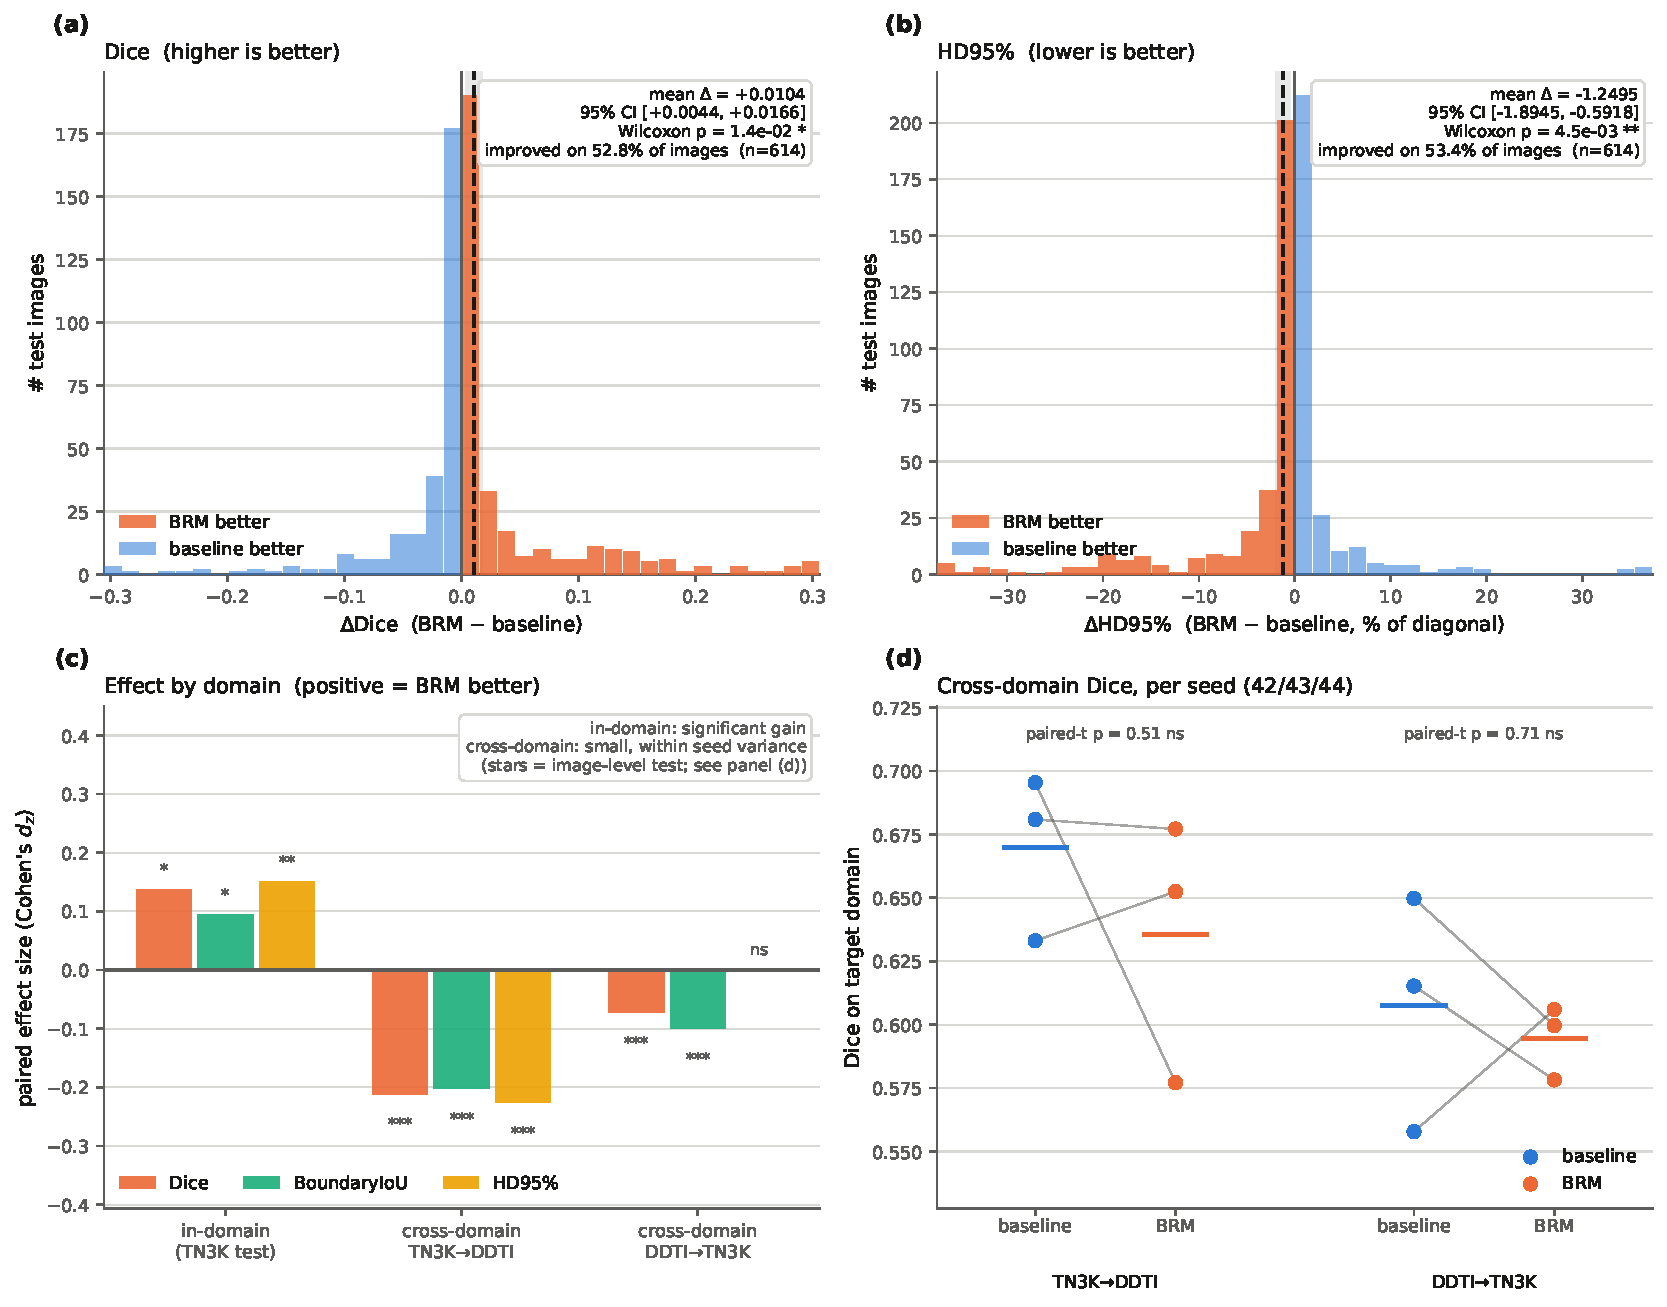
\includegraphics[width=0.97\linewidth]{fig9_significance_2x2}
  \caption[통계적 유의성과 교차 데이터셋 결과.]{통계적 유의성과 교차 데이터셋 결과. (a)(b) 영상별 대응 차이의 분포 — 점선은 평균, 회색 띠는 95\%
    신뢰구간. (c) 설정별 효과크기 $d_z$. (d) LODO 시드별 Dice — 같은 시드끼리 선으로 이었다.}
  \label{fig:significance}
\end{figure}

\paragraph{영상 단위.} 세 경계 지표 모두 유의하였다. Dice의 평균 차이는 +0.0104(95\% CI [+0.0044, +0.0166],
Wilcoxon $p$=0.014), Boundary IoU는 +0.0055([+0.0009, +0.0102], $p$=0.011), HD95는 $-$1.25\%p([$-$1.89, $-$0.59],
$p$=0.0045)였다. 세 신뢰구간 모두 0을 포함하지 않는다. 효과크기는 $d_z$=0.09--0.15로 작은 편이다.

개선 비율이 52.8--53.6\%로 절반을 조금 넘는다는 점은 해석에 중요하다. \figref{fig:significance}(a)(b)에서 보듯
대부분의 영상에서는 두 모델의 차이가 0 근처에 몰려 있고, 평균 개선은 일부 영상에서의 큰 개선에서 나온다.
즉 제안 방법은 모든 영상을 조금씩 낫게 만들기보다, 베이스라인이 경계를 크게 놓치던 일부 영상을 바로잡는 방식으로
작동한다.

\paragraph{fold 단위.} 5개 fold의 평균을 짝지은 검정에서는 세 지표 모두 유의하지 않았다(Wilcoxon $p$=0.0625,
0.1875, 0.3125). 그러나 n=5에서 양측 Wilcoxon 검정이 도달할 수 있는 최소 $p$가 0.0625이므로, Dice의 $p$=0.0625는
5개 fold가 모두 같은 방향으로 개선되었을 때 나올 수 있는 가장 강한 결과이다. 효과크기도 $d_z$=0.71--1.09로 크다.
fold 단위의 '유의하지 않음'은 효과가 없다는 증거가 아니라 표본 5개의 검정력 한계로 읽어야 한다.

이상의 결과로 \textbf{H2는 지지된다}. 경계 지표의 개선은 영상 단위에서 통계적으로 유의하고, 추론 연산량은
늘지 않았다.

\section{교차 데이터셋 일반화}\label{sec:exp_lodo}

마지막으로 제안 방법의 효과가 학습하지 않은 데이터셋에서도 유지되는지 LODO로 확인하였다(\tabref{tab:lodo}).
처음에는 시드 42 하나로 실험하였으나, 결과의 변동이 커서 시드 43, 44를 추가로 학습하여 세 시드로 반복하였다.

% 자동 생성 파일 — scripts/make_thesis.py 가 덮어쓴다. 직접 고치지 말 것.
\begin{table}[htbp]
\centering
\small
\caption[교차 데이터셋(LODO) 결과 — 3개 시드(42, 43, 44) 평균 $\pm$ 표준편차.]{교차 데이터셋(LODO) 결과 — 3개 시드(42, 43, 44) 평균 $\pm$ 표준편차. Mask mAP는 저장된 체크포인트(검증 fitness 최대 epoch)의 값이며, 경계 지표는 타깃 도메인 전체 영상에 대한 평균이다. $p$는 시드 단위 대응 $t$ 검정(n=3)이다.}
\label{tab:lodo}
\begin{adjustbox}{max width=\linewidth}
\begin{tabular}{llcccc}
\toprule
방향 & 지표 & 베이스라인 & 제안 (BRM) & $\Delta$ & 시드 단위 $p$ \\
\midrule
\multirow{4}{*}{TN3K$\rightarrow$DDTI} & Mask mAP$_{50:95}$ & 0.4465 $\pm$ 0.0136 & 0.4365 $\pm$ 0.0056 & -0.0100 & 0.454 (n.s.) \\
 & Dice & 0.6698 $\pm$ 0.0326 & 0.6356 $\pm$ 0.0521 & -0.0342 & 0.506 (n.s.) \\
 & HD95 (\%) & 21.372 $\pm$ 4.245 & 25.810 $\pm$ 7.522 & +4.438 & 0.532 (n.s.) \\
 & Boundary IoU & 0.2722 $\pm$ 0.0022 & 0.2549 $\pm$ 0.0105 & -0.0173 & 0.073 (n.s.) \\
\midrule
\multirow{4}{*}{DDTI$\rightarrow$TN3K} & Mask mAP$_{50:95}$ & 0.3146 $\pm$ 0.0210 & 0.3015 $\pm$ 0.0042 & -0.0131 & 0.444 (n.s.) \\
 & Dice & 0.6076 $\pm$ 0.0465 & 0.5946 $\pm$ 0.0145 & -0.0130 & 0.714 (n.s.) \\
 & HD95 (\%) & 23.173 $\pm$ 4.875 & 23.169 $\pm$ 1.769 & -0.004 & 0.999 (n.s.) \\
 & Boundary IoU & 0.2285 $\pm$ 0.0231 & 0.2189 $\pm$ 0.0166 & -0.0096 & 0.693 (n.s.) \\
\bottomrule
\end{tabular}
\end{adjustbox}
\end{table}


\paragraph{단일 시드의 결과.} 시드 42만 보면 TN3K$\rightarrow$DDTI에서 제안 모델의 Dice가 0.6954에서 0.5771로
0.118 떨어지고 HD95가 17.89\%에서 34.15\%로 거의 두 배가 되어, 제안 방법이 교차 데이터셋에서 크게 악화되는
것처럼 보였다(\tabref{tab:lodo_seed}). 이 차이는 637장 영상 단위 검정에서 $p<10^{-10}$으로 매우 유의하였다.

\paragraph{세 시드의 결과.} 그러나 시드를 늘리자 그림이 달라졌다. 시드 43, 44에서 제안 모델의 Dice는 0.6771,
0.6525로 베이스라인(0.6809, 0.6331)과 비슷하거나 오히려 높았고, 시드 42의 제안 모델(0.5771)이 이상치였음이
드러났다. 세 시드 평균의 차이는 TN3K$\rightarrow$DDTI에서 Dice $-$0.034, DDTI$\rightarrow$TN3K에서 $-$0.013으로
줄었고, 시드 단위 검정에서는 모든 지표가 유의하지 않았다($p$=0.073--0.999). 무엇보다 시드 간 표준편차
(Dice 기준 0.015--0.052)가 두 모델의 차이보다 크다. 즉 현재의 표본으로는 차이가 제안 방법 때문인지 실행 간
변동 때문인지 구분할 수 없다.

Mask \mAP{} 역시 두 방향 모두 제안 모델이 0.010--0.013 낮았으나 유의하지 않았다($p$=0.454, 0.444).
유일하게 일관된 신호는 TN3K$\rightarrow$DDTI의 Boundary IoU로, 세 시드 모두 제안 모델이 낮았다($\Delta$=$-$0.017,
$p$=0.073). 이 역시 유의수준에 이르지 않으므로 '약한 경향' 이상으로 해석하지 않는다.

정리하면, 경계 정교화의 효과는 학습 분포 안에서는 유의하지만 교차 데이터셋에서는 유지되지 않으며,
그렇다고 악화가 확인된 것도 아니다. \textbf{교차 데이터셋 일반화는 현재의 표본으로 판정할 수 없다}.
이 결과의 해석은 \secref{sec:disc_lodo}에서 다룬다.

\section{경량화 결과 (H3)}\label{sec:exp_quant}

\tabref{tab:quant}와 \figref{fig:quantization}은 제안 모델의 정밀도별 결과이다.

% 자동 생성 파일 — scripts/make_thesis.py 가 덮어쓴다. 직접 고치지 말 것.
\begin{table*}[htbp]
\centering
\footnotesize
\caption[정밀도별 경량화 결과 (제안 모델, held-out TN3K test, 5-fold 평균 $\pm$ 표준편차).]{정밀도별 경량화 결과 (제안 모델, held-out TN3K test, 5-fold 평균 $\pm$ 표준편차). 지연 시간은 batch 1, 640$\times$640 입력, 워밍업 15회 후 100회 평균의 fold 평균이며 fold 간 표준편차는 CPU 0.02--4.86 ms, GPU 0.05 ms 이하였다. INT8 모델의 정확도는 CPU에서 측정했다.}
\label{tab:quant}
\setlength{\tabcolsep}{3.5pt}
\begin{adjustbox}{max width=\linewidth}
\begin{tabular}{lccccccc}
\toprule
정밀도 & 크기 (MB) & CPU (ms) & GPU (ms) & Mask mAP$_{50:95}$ & Dice & HD95 (\%) & BIoU \\
\midrule
PyTorch FP32 & 6.01 & -- & -- & 0.6267 $\pm$ 0.0081 & 0.8300 $\pm$ 0.0039 & 8.378 $\pm$ 0.775 & 0.4414 $\pm$ 0.0050 \\
ONNX FP32 & 11.63 & 62.82 & 3.53 & 0.6188 $\pm$ 0.0077 & 0.8300 $\pm$ 0.0049 & 8.529 $\pm$ 0.899 & 0.4402 $\pm$ 0.0056 \\
ONNX FP16 & 5.87 & -- & 3.13 & 0.6194 $\pm$ 0.0080 & 0.8301 $\pm$ 0.0050 & 8.516 $\pm$ 0.911 & 0.4403 $\pm$ 0.0058 \\
ONNX Runtime INT8 & 5.45 & 44.00 & -- & 0.6032 $\pm$ 0.0160 & 0.8184 $\pm$ 0.0123 & 9.395 $\pm$ 1.026 & 0.4299 $\pm$ 0.0121 \\
\textbf{OpenVINO INT8} & \textbf{3.71} & \textbf{4.10} & \textbf{--} & \textbf{0.6161 $\pm$ 0.0085} & \textbf{0.8290 $\pm$ 0.0051} & \textbf{8.497 $\pm$ 0.706} & \textbf{0.4379 $\pm$ 0.0075} \\
\bottomrule
\end{tabular}
\end{adjustbox}
\end{table*}


\begin{figure}[htbp]
  \centering
  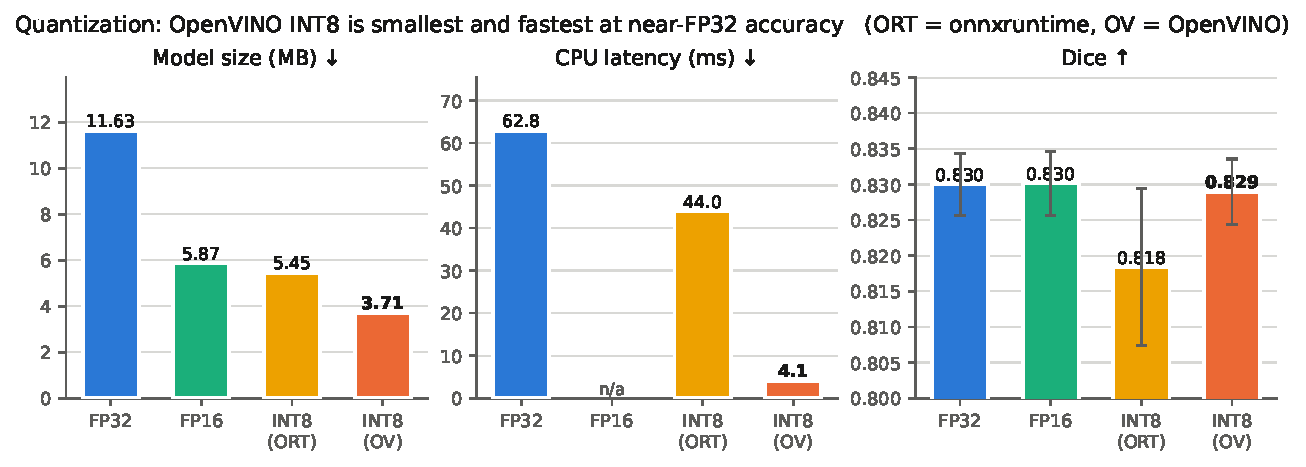
\includegraphics[width=\linewidth]{fig3_quantization}
  \caption[정밀도별 모델 크기, CPU 지연, Dice.]{정밀도별 모델 크기, CPU 지연, Dice. ORT = ONNX Runtime, OV = OpenVINO.}
  \label{fig:quantization}
\end{figure}

\paragraph{FP32와 FP16.} ONNX FP32는 Dice 0.8300으로 PyTorch와 같았고, Mask \mAP{}는 0.6188로 0.008 낮았다.
경계 지표가 그대로라는 점에서 마스크 자체의 품질보다는 검증 절차에서 ONNX 예측을 처리하는 방식의 차이일 가능성이
있으나, 원인은 확인하지 못하였다. FP16은 FP32와 정확도가 같으면서 크기가
절반(5.87 MB)이고 GPU 지연이 3.53 ms에서 3.13 ms로 줄어, GPU 배포에서는 손실 없는 선택이다.

\paragraph{INT8.} 두 INT8 경로의 결과는 크게 달랐다. ONNX Runtime INT8은 CPU 지연이 44.00 ms로 FP32(62.82 ms)보다
30\% 빨라지는 데 그쳤고, 정확도도 Mask \mAP{} 0.6032, Dice 0.8184로 가장 많이 떨어졌다. 반면 OpenVINO INT8은
3.71 MB로 가장 작으면서 CPU 지연 4.10 ms로 FP32보다 15.3배, ONNX Runtime INT8보다 10.7배 빨랐다.
정확도 손실은 Dice 0.001, Mask \mAP{} 0.003(ONNX FP32 대비)에 그쳤고 HD95는 8.497\%로 오히려 FP32(8.529\%)보다
조금 나았다. fold 간 지연의 표준편차도 0.02 ms로 가장 안정적이었다.

\figref{fig:pareto}는 정확도와 CPU 지연의 절충을 한눈에 보여 준다. OpenVINO INT8은 지연, 크기, 정확도 모두에서
다른 CPU 후보를 앞서는 지배적 선택이다.

\begin{figure}[htbp]
  \centering
  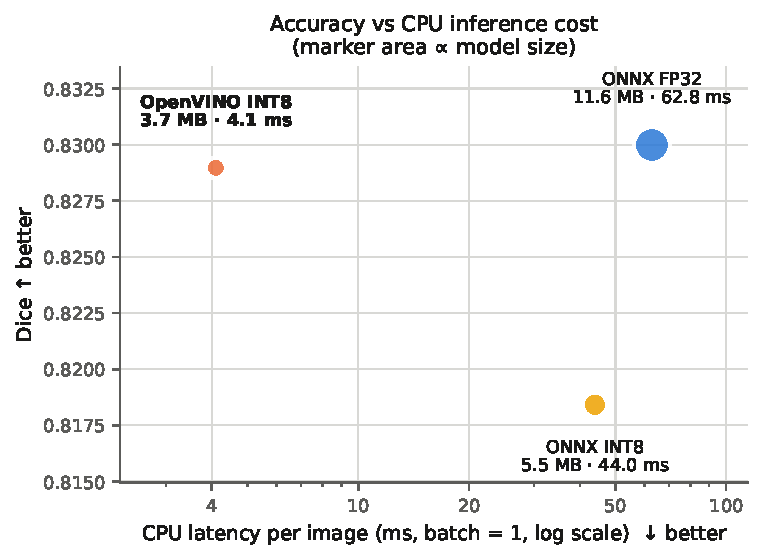
\includegraphics[width=0.62\linewidth]{fig2_accuracy_vs_latency}
  \caption[CPU 지연과 Dice의 절충.]{CPU 지연과 Dice의 절충. 마커 넓이는 모델 파일 크기에 비례한다. 가로축은 로그 척도이다.}
  \label{fig:pareto}
\end{figure}

OpenVINO INT8은 CPU에서 영상 한 장을 4.10 ms에 처리하므로 순전파만으로는 초당 약 240장을 처리할 수 있으며, Dice 손실은
fold 표준편차(0.005)보다 작다. 따라서 \textbf{H3은 OpenVINO INT8 경로에서 지지된다}. ONNX Runtime INT8 경로는
지연과 정확도 모두에서 기준에 미치지 못하므로, 같은 'INT8 사후 양자화'라도 변환 도구에 따라 결론이 달라진다는
점을 함께 밝혀 둔다.

\section{단계별 누적 결과}\label{sec:exp_final}

\tabref{tab:final}은 베이스라인에서 최종 배포 모델까지의 누적 변화이다.

% 자동 생성 파일 — scripts/make_thesis.py 가 덮어쓴다. 직접 고치지 말 것.
\begin{table*}[htbp]
\centering
\footnotesize
\caption[단계별 누적 결과 (held-out TN3K test, 5-fold 평균).]{단계별 누적 결과 (held-out TN3K test, 5-fold 평균). PyTorch 모델의 지연 시간은 배포 형식과 측정 조건이 달라 비교에서 제외했다.}
\label{tab:final}
\begin{adjustbox}{max width=\linewidth}
\begin{tabular}{lccccccc}
\toprule
모델 & Mask mAP$_{50:95}$ & Dice & HD95 (\%) & BIoU & 크기 (MB) & CPU (ms) & GPU (ms) \\
\midrule
베이스라인 nano & 0.6272 & 0.8195 & 9.628 & 0.4358 & 6.00 & -- & -- \\
+ 경계 정교화 & 0.6267 & 0.8300 & 8.378 & 0.4414 & 6.01 & -- & -- \\
+ ONNX FP16 & 0.6194 & 0.8301 & 8.516 & 0.4403 & 5.87 & -- & 3.13 \\
+ ONNX Runtime INT8 & 0.6032 & 0.8184 & 9.395 & 0.4299 & 5.45 & 44.00 & -- \\
\textbf{+ OpenVINO INT8 (최종)} & \textbf{0.6161} & \textbf{0.8290} & \textbf{8.497} & \textbf{0.4379} & \textbf{3.71} & \textbf{4.10} & \textbf{--} \\
\bottomrule
\end{tabular}
\end{adjustbox}
\end{table*}


경계 정교화로 얻은 개선은 양자화를 거친 뒤에도 대부분 유지되었다. 최종 OpenVINO INT8 모델은 베이스라인
PyTorch 모델과 비교하여 Dice +0.0095(0.8195$\rightarrow$0.8290), HD95 $-$11.7\%(9.628$\rightarrow$8.497),
Boundary IoU +0.0021을 유지하면서, 파일 크기는 6.00 MB에서 3.71 MB로 줄고 CPU에서 4.10 ms에 동작한다.
Mask \mAP{}는 0.6272에서 0.6161로 0.011 낮아졌는데, 대부분 PyTorch에서 ONNX로 바꿀 때 생긴 차이(0.008)이다.

% ============================================================================
\chapter{논의}\label{ch:discussion}
% ============================================================================

\section{가설 검증 요약}\label{sec:disc_summary}

\tabref{tab:hypotheses}는 \secref{sec:hypothesis}에서 세운 세 가설의 검증 결과이다.

\begin{table}[htbp]
\centering\small
\caption{가설 검증 요약.}
\label{tab:hypotheses}
\begin{tabular}{p{0.1\linewidth}p{0.47\linewidth}p{0.14\linewidth}p{0.18\linewidth}}
\toprule
가설 & 핵심 근거 & 판정 & 남은 단서 \\
\midrule
H1 & nano Mask \mAP{} 0.6272, small 0.6239. 차이는 fold 표준편차 이내이고 small은 3.5배 크다. & 지지 & -- \\
H2 & 영상 단위 검정에서 Dice·BIoU·HD95 모두 유의($p\le0.014$). 추론 GFLOPs 동일(9.73). & 지지 &
  개선 폭은 계수 선택 편향 가능성(\secref{sec:sweep}), 교차 데이터셋은 판정 불가 \\
H3 & OpenVINO INT8: 3.71 MB, CPU 4.10 ms(15.3배), Dice 손실 0.001. & 지지 (OpenVINO) &
  ONNX Runtime INT8은 기준 미달 \\
\bottomrule
\end{tabular}
\end{table}

\section{mAP가 경계 개선을 반영하지 못하는 이유}\label{sec:disc_map}

제안 모델은 경계 지표를 유의하게 개선했지만 Mask \mAP{}는 0.6272에서 0.6267로 거의 변하지 않았다.
이는 지표의 구조로 설명할 수 있다. \secref{sec:disc_lambda}에서 계산하듯 경계 밴드는 결절 상자 안 픽셀의 약 16\%에
불과하므로, 경계 부근이 몇 픽셀 개선되어도 마스크 IoU는 조금밖에 변하지 않는다. mAP는 이 IoU가 0.50, 0.55, \dots, 0.95의
임계값을 넘는지만 세므로, IoU가 임계값을 넘나들지 않는 한 개선이 점수에 나타나지 않는다. 게다가 mAP는 검출 순위와
상자 품질에도 크게 좌우된다.

반면 HD95는 경계의 최악 오차를, Boundary IoU는 경계 띠에서의 겹침만을 재므로 같은 변화에 훨씬 민감하다.
\secref{sec:exp_sig}에서 개선이 일부 영상의 큰 개선에서 나온다는 점을 보였는데, 바로 그런 영상, 즉 베이스라인의 경계가
음영 구간으로 새어 나가던 영상에서 HD95가 크게 줄었다. 이 결과는 \secref{sec:problem}의 P1, 즉 영역 지표만으로는
경계 품질을 판정할 수 없다는 문제 정의를 실험적으로 뒷받침한다.

\section{경계 강조 계수의 해석}\label{sec:disc_lambda}

스윕에서 $\lambda=2$는 $\lambda=10$보다 HD95에서 일관되게 나았다. 경계를 더 강하게 강조할수록 경계가 좋아지리라는 직관과
반대되는 결과이며, \eqnref{eq:weight}의 가중치가 정규화되지 않는다는 점에서 원인을 찾을 수 있다.

가중치 $w_p = 1 + \lambda\mathcal{B}_p$는 모든 픽셀에서 1 이상이므로, $\lambda$를 키우면 경계 픽셀의 상대적 비중이 커지는 동시에
마스크 손실 전체의 크기도 커진다. 정답 상자 안에서 경계 밴드가 차지하는 비율을 $\rho$라 하면 상자 안 평균 가중치는
$\mathbb{E}[w] = 1 + \lambda\rho$이다. 학습 데이터의 결절 3,767개를 640 레터박스 후 마스크 해상도(1/4)로 래스터화하여 계산한
$\rho$의 중앙값은 TN3K 16.3\%, DDTI 17.0\%였다. 이에 따르면 $\lambda=2$에서 마스크 손실은 평균 약 1.33배, $\lambda=10$에서는
약 2.64배(사분위 범위 2.09--3.46배)로 커진다. 학습 중 모자이크와 스케일 증강으로 결절의 크기가 바뀌므로 정확한 값은 다르지만,
$\lambda=10$이 마스크 손실을 두 배 이상 키운다는 점은 달라지지 않는다.

즉 $\lambda$는 '경계 강조'와 '분할 손실의 전체 가중치'라는 두 가지를 함께 바꾼다. $\lambda=10$에서는 분할 손실이 상자·분류
손실보다 과도하게 커져 \eqnref{eq:total_loss}의 손실 균형이 흐트러지고, 이것이 Mask \mAP{} 하락과 경계 개선 폭의 감소로
나타난 것으로 해석된다. 초기값 $\lambda=5$에서 mAP가 떨어졌던 것(0.627$\rightarrow$0.621)도 같은 맥락이다.
후속 연구에서는 $w$를 $\mathbb{E}[w]$로 나누어 손실 크기를 고정하고 경계의 상대 비중만 바꾸는 정규화를 적용하면,
두 효과를 분리하여 $\lambda$를 더 넓은 범위에서 탐색할 수 있을 것이다.

\section{교차 데이터셋 결과의 해석}\label{sec:disc_lodo}

\subsection{성능이 낮은 이유: 데이터의 차이}

LODO에서는 베이스라인과 제안 모델 모두 in-domain보다 성능이 크게 낮았다(Mask \mAP{} 0.30--0.45 대 0.63). 특히
DDTI$\rightarrow$TN3K 방향이 낮았는데, \secref{sec:ds_gap}의 분석이 그 이유를 설명한다. DDTI는 637장으로 작고,
모든 영상이 단일 결절이며, 결절 크기가 영상의 1.5--24\%에 몰려 있다. 이 데이터만으로 학습한 모델은 평가 대상인 TN3K 전체 3,493장 중
8.4\%(294장)를 차지하는 다중 결절 영상과, 영상의 1\% 미만인 작은 결절 또는 40\%를 넘는 큰 결절을 학습한 적이 없다.
영상 형식도 다르다. DDTI는 장비 화면 전체를 담고 있어 결절 주변에 UI 요소가 함께 있는 반면, TN3K는 결절 주변을
잘라낸 확대 영상이다. 따라서 LODO의 낮은 성능은 모델 구조의 결함이라기보다 학습 데이터가 평가 분포를 포함하지
못한 결과로 보는 것이 타당하다.

\subsection{경계 정교화의 효과가 사라진 이유}

in-domain에서 유의했던 경계 개선이 LODO에서 사라진 데에는 두 가지 해석이 가능하다. 하나는 경계 가중 손실이
학습 데이터의 주석 경계에 더 강하게 맞추도록 하므로, 주석 방식이 다른 데이터셋에서는 그 이득이 줄어든다는 것이다.
TN3K$\rightarrow$DDTI의 Boundary IoU가 세 시드 모두에서 제안 모델이 낮았던 점은 이 해석과 어울린다. 다른 하나는
도메인 이동으로 결절 자체를 놓치거나 엉뚱한 영역을 잡는 큰 오류가 늘어나, 경계 몇 픽셀의 개선이 그 오류에 묻혔다는
것이다. LODO에서 HD95가 20\%를 넘는다는 것은 경계 정밀도보다 검출 자체의 실패가 지배적이라는 뜻이다.
현재의 실험으로는 두 해석을 구분할 수 없다.

\subsection{단일 실행으로 결론을 내리면 안 되는 이유}

본 연구의 교차 데이터셋 결과는 실행 간 변동의 중요성을 잘 보여 준다. 시드 42 하나만 보면 TN3K$\rightarrow$DDTI에서
제안 모델의 Dice가 0.118 떨어졌고, 637장 영상 단위 검정의 $p$값은 $10^{-10}$보다 작았다. 이 결과만으로 논문을 썼다면
"경계 정교화는 교차 도메인에서 성능을 크게 해친다"는 강한 결론을 내렸을 것이다. 그러나 시드 두 개를 더하자 그 차이는
대부분 시드 42의 제안 모델 한 번의 실행에서 나온 것으로 드러났다.

여기서 영상 단위 검정과 시드 단위 검정이 답하는 질문이 다르다는 점이 중요하다. 영상 단위 검정은 이미 학습된 특정 모델들을
고정하고 테스트 영상의 표본 변동만 오차로 삼으므로, "이 두 모델 중 어느 쪽이 새 영상에서 나은가"에 답한다. 학습을 다시 하면
달라질 수 있는 부분, 즉 학습의 무작위성은 오차에 포함되지 않는다. 반면 "이 학습 방법이 다른 방법보다 나은가"라는 기법에
관한 질문은 학습을 반복했을 때의 변동을 오차로 삼아야 하며, 이를 반영하는 것이 시드 단위 검정이다\citep{bouthillier2021variance}.
in-domain 결과에서도 같은 구분이 적용된다. 영상 단위 검정이 유의하고 5개 fold 모두에서 Dice가 개선되었다는 점은 강한 근거이지만,
fold 단위 검정은 검정력 한계로 유의수준에 이르지 못했으므로(\secref{sec:exp_sig}), 기법의 효과를 확정하려면 더 많은 반복이
도움이 된다.

\section{양자화 결과의 해석}\label{sec:disc_quant}

두 INT8 경로의 CPU 지연이 44.00 ms와 4.10 ms로 10배 이상 차이 난 가장 큰 원인은 양자화에서 제외된 연산의 범위이다.
제안 모델의 추론 그래프에서 합성곱 연산량을 층별로 집계하면, 백본이 31.8\%, 넥이 16.4\%, 분할 헤드가 51.8\%를 차지한다.
헤드의 비중이 큰 이유는 프로토타입 경로가 입력의 1/4 해상도(160$\times$160)에서 64채널 3$\times$3 합성곱을 수행하기
때문으로, 프로토타입 경로 하나가 전체의 27.9\%이다.

ONNX Runtime 경로는 출력 붕괴를 막기 위해 헤드 전체를 부동소수점으로 남겼으므로, 연산량의 절반 이상이 양자화되지
않았다. 양자화된 나머지 48\%가 아무리 빨라져도 전체 지연은 헤드의 부동소수점 연산 시간 아래로 내려갈 수 없다.
여기에 양자화된 구간과 부동소수점 구간의 경계마다 정수와 실수를 오가는 변환 연산이 추가된다. 그 결과 지연이 FP32 대비
30\% 줄어드는 데 그쳤다. 반면 OpenVINO 경로는 헤드의 합성곱은 양자화하고 시그모이드, DFL, 원소별 산술 연산만
부동소수점으로 남겼다. 출력 붕괴를 일으키는 민감한 연산만 골라 제외하고 연산량의 대부분은 정수로 옮긴 것이다.
OpenVINO 런타임이 CPU의 정수 벡터 명령에 맞춰 연산을 최적화한다는 점도 기여했을 것이나, 그 몫을 분리하지는 않았다.

정확도 측면에서도 OpenVINO 경로가 나았다(Dice 0.8290 대 0.8184). 두 경로 모두 가중치는 대칭, 활성값은 비대칭으로 양자화하므로
기본 방식은 비슷하다. 그러나 캘리브레이션 데이터(TN3K 학습·검증 150장 대 fold별 검증 분할), 양자화 제외 범위, NNCF가 기본으로
수행하는 편향 보정 등 여러 요인이 함께 다르므로, 정확도 차이를 한 요인으로 돌리기는 어렵다. 이 비교에서 얻을 수 있는 실무적 교훈은, 같은 'INT8 사후 양자화'라는
이름 아래서도 어떤 연산을 어떻게 제외하느냐가 결과를 결정한다는 것이다.

\section{연구의 한계}\label{sec:limitations}

본 연구의 결과는 다음 한계 안에서 해석해야 한다.

\begin{enumerate}
  \item \textbf{계수 선택 편향.} 경계 손실 계수는 held-out 집합의 결과로 선택되었다(\secref{sec:sweep}). 사후 점검에서
    경계 정교화의 효과 자체는 검증 분할에서도 재현되었지만, 채택한 구성의 우위는 재현되지 않았다. 따라서 최종 모델의
    개선 폭은 낙관적일 수 있다. 검증 분할에서 가장 나았던 구성($g=0.25$, $\lambda=2$)을 전체 fold에서 다시 학습하여
    held-out에서 평가하면 이 편향 없이 효과를 추정할 수 있다.
  \item \textbf{작은 효과크기.} 경계 개선의 효과크기는 $d_z\approx0.1$--0.15로 작다. 통계적으로 유의한 차이가
    판독에 의미 있는 차이인지는 검증하지 않았다.
  \item \textbf{교차 데이터셋 결과의 낮은 검정력.} 시드 3개로는 작은 효과를 검출하기 어렵다. 교차 데이터셋에서
    개선도 악화도 확인되지 않았다는 결과는 '효과가 없다'가 아니라 '판정할 수 없다'로 읽어야 한다.
  \item \textbf{LODO의 낙관적 평가.} LODO에서는 타깃 데이터셋을 검증 집합으로도 사용하여 체크포인트를 골랐으므로,
    두 모델의 비교는 공정하지만 절대값은 실제 미지 도메인의 성능보다 높을 수 있다.
  \item \textbf{학습 무작위성의 부분적 반영.} in-domain 실험은 fold마다 시드 42로 한 번씩 학습하였다. fold 간 변동이
    학습 무작위성의 일부를 반영하지만, 같은 fold를 여러 시드로 반복하지는 않았다.
  \item \textbf{지연 측정 환경.} CPU 지연은 96코어 서버 CPU(AMD EPYC 9654)에서 측정하였다. 휴대형 장비나 일반 판독 PC의
    저전력 CPU에서는 절대값이 크게 다를 것이며, 정밀도 간 상대 순위도 달라질 수 있다.
  \item \textbf{범위의 제한.} 하나의 구조(YOLOv11n-seg), 단일 병변 클래스, 두 공개 데이터셋에 한정된 결과이다.
    임상 기관에서 새로 수집한 외부 데이터로는 검증하지 않았다.
\end{enumerate}

% ============================================================================
\chapter{결론}\label{ch:conclusion}
% ============================================================================

\section{연구 요약}

본 연구는 갑상선 결절 초음파 영상에서 경계 정확도를 높이면서 CPU에서 실시간으로 동작하는 검출·분할
모델을 목표로, YOLOv11-seg를 기반으로 데이터 혼합, 경계 정교화, 사후 양자화를 하나의 파이프라인에서
검증하였다. 세 가설의 검증 결과는 다음과 같다.

\begin{enumerate}
  \item \textbf{경량 백본에서 출발해도 손해가 없다 (H1 지지).} YOLOv11n-seg는 small 대비 파라미터 1/3.5,
    연산량 1/3.4임에도 held-out Mask \mAP{}가 0.6272로 small(0.6239)과 동등하였다. 결절이라는 단일
    클래스 과제에서 큰 모델의 추가 용량은 정확도로 이어지지 않았다.

  \item \textbf{경계 정교화를 추론 비용 없이 얻을 수 있다 (H2 지지).} 학습 전용 경계 분기와 경계 가중 손실로
    Dice가 0.8195에서 0.8300으로, HD95가 9.628\%에서 8.378\%로(13.0\% 감소), Boundary IoU가 0.4358에서
    0.4414로 개선되었고, 세 지표 모두 영상 단위 대응표본 검정에서 유의하였다. 추론 연산량은 9.73 GFLOPs로
    베이스라인과 같았다. 다만 손실 계수를 held-out 결과로 고른 탓에 이 개선 폭은 낙관적일 수 있으며,
    검증 분할로 다시 점검했을 때 경계 개선 자체는 모든 계수 구성에서 재현되었다.

  \item \textbf{CPU 배포가 실용 범위에 들어왔다 (H3 지지, 변환 도구에 따라 다름).} OpenVINO INT8 모델은 3.71 MB,
    CPU 지연 4.10 ms로 ONNX FP32 대비 15.3배 빨랐고 Dice 손실은 0.001에 그쳤다. 반면 ONNX Runtime INT8은
    검출 헤드를 부동소수점으로 남겨야 해 44.00 ms에 머물렀고 Dice도 0.012 떨어졌다.
\end{enumerate}

교차 데이터셋 조건에서는 경계 개선이 유지되지 않았다. 다만 3개 시드로 반복하자 악화 역시 통계적으로
확인되지 않았으므로, 본 연구는 교차 데이터셋 일반화에 대해 판단을 유보한다. 단일 실행 결과만 보았다면
"교차 도메인에서 크게 악화된다"는 잘못된 결론을 내렸을 것이며, 이를 시드 반복으로 바로잡은 과정 자체도
본 연구가 남기는 교훈이다.

\section{향후 연구}

\paragraph{오검출 실패 유형의 억제.} 정성 분석의 최악 사례(\figref{fig:qualitative})처럼 제안 모델이
주변 조직을 결절로 포함하는 경우가 있었다. 경계 가중이 잘못 잡힌 경계를 오히려 강화했을 가능성이 있으므로,
예측 경계의 불확실성을 함께 추정하거나 오검출에 별도 벌점을 주는 손실을 검토할 필요가 있다.

\paragraph{도메인 이동 대응.} \chapref{ch:dataset}의 분석은 두 데이터셋의 차이가 영상 형식(장비 화면
캡처와 확대 영상), 결절 크기 분포, 결절 수에서 모두 크다는 것을 보여 준다. DDTI의 장비 UI 영역을
가리거나 잘라내는 전처리, 스타일 정규화, 도메인 적대 학습\citep{ganin2015dann}을 결합하여 교차 데이터셋
성능을 다시 검증할 필요가 있다. 또한 더 많은 시드와 제3의 외부 데이터셋을 확보하면 일반화 여부를
판정할 수 있는 검정력을 얻을 수 있다.

\paragraph{양자화 인식 학습.} ONNX Runtime INT8에서 나타난 정확도 손실은 사후 양자화의 한계일 수 있다.
양자화 인식 학습으로 헤드까지 정수 연산으로 옮기면서 정확도를 회복할 수 있는지 확인할 가치가 있다.

\paragraph{실제 배포 장비에서의 측정.} 본 연구의 CPU 지연은 96코어 서버 CPU에서 측정한 값이다.
휴대형 초음파나 판독 PC에 쓰이는 저전력 x86·ARM CPU, Jetson 같은 임베디드 장비에서 지연과 전력을
실측해야 배포 가능성을 확정할 수 있다.

\paragraph{임상적 유용성 검증.} 경계 지표의 개선이 판독에 의미 있는 차이인지는 별도로 확인해야 한다.
예측 경계로부터 TI-RADS 경계 범주(매끄러움, 분엽상, 불규칙)를 자동 판정하고, 그 일치도를 전문의 판독과
비교하는 연구로 확장할 수 있다.


% ── 뒷부분 ───────────────────────────────────────────────────────────
\cleardoublepage
\phantomsection\addcontentsline{toc}{chapter}{\bibname}
\bibliographystyle{unsrtnat}
\bibliography{refs}

\appendix
% ============================================================================
% 부록
% ============================================================================

\chapter{재현 절차}\label{app:repro}

본 연구의 모든 코드와 수치 결과는 연구 저장소에 있다. 원본 데이터셋 영상과 모델 가중치는 용량과 재배포
문제로 저장소에 포함하지 않았다. 아래 명령은 저장소 최상위에서 실행한다.

\section{환경 구성}

\begin{small}
\begin{verbatim}
# 1) ultralytics 기반 커밋에 본 연구의 변경분(패치)을 적용
git clone https://github.com/ultralytics/ultralytics.git ultralytics_thyroid
cd ultralytics_thyroid
git checkout 4dcc98a6be09d058c206f2756f3ee2966d1c4b71
git apply ../ultralytics_patches/thyroid.patch
pip install -e . && cd ..
# 2) 부가 의존성
pip install onnx onnxruntime-gpu openvino nncf scipy
\end{verbatim}
\end{small}

패치는 \BRM{} 헤드(\texttt{nn/modules/head.py}), 경계 인식 손실(\texttt{utils/loss.py}), 모델 구성 파일
(\texttt{cfg/models/11/yolo11-seg-brm.yaml})과 이들의 등록 코드를 담고 있다. 경계 손실 계수는 환경 변수
\texttt{BRM\_HEAD\_GAIN}($g$, 기본 1.0)과 \texttt{BRM\_LAMBDA}($\lambda$, 기본 2.0)로 바꿀 수 있다.

\section{실행 순서}

\begin{small}
\begin{verbatim}
python scripts/convert_to_yoloseg.py        # 마스크 -> YOLO-seg 다각형 (3.4절)
python scripts/make_splits.py               # 5-fold / LODO / held-out 분할 (3.5절)
bash   scripts/run_baseline_rest.sh         # 베이스라인 nano·small 학습 (5.4절)
bash   scripts/run_phase3_sweep.sh          # 경계 손실 계수 스윕 (5.5절)
python scripts/sweep_eval.py                # 스윕 결과표, held-out 기준 (5.5절)
python scripts/sweep_eval.py --split val    # 같은 모델의 검증 분할 기준 사후 점검
bash   scripts/run_phase3_final.sh          # 제안 모델 5-fold + LODO 학습 (5.6절)
bash   scripts/run_lodo_seeds.sh            # LODO 시드 43·44 반복 (5.9절)
python scripts/stats_test.py --part all     # 대응표본 검정 (5.8절, 5.9절)
python scripts/export_quant.py --fold N     # 정밀도별 변환, N = 0..4 (4.6절)
python scripts/eval_quant.py --folds 0,1,2,3,4   # 정밀도별 평가 (5.10절)
python scripts/final_table.py               # 단계별 누적 결과 (5.11절)
python scripts/make_thesis.py --zip         # 본 논문의 표·그림 재생성
\end{verbatim}
\end{small}

학습 스크립트는 같은 이름의 출력 폴더를 덮어쓰며 이어 쓰도록 설정되어 있어, 같은 실행을 두 번 띄우면
두 학습의 기록과 가중치가 섞인다. 실제로 이 문제로 제안 모델의 fold 0--2 결과가 오염된 적이 있어, 해당 fold를
처음부터 다시 학습하였고 재실행 스크립트에 기존 폴더가 있으면 실행을 거부하는 장치를 넣었다
(\appref{app:impl}). 평가는 반드시 학습 드라이버의 종료 기록을 확인한 뒤 수행해야 한다.

\chapter{상세 결과}\label{app:detail}

\section{fold별 결과}
% 자동 생성 파일 — scripts/make_thesis.py 가 덮어쓴다. 직접 고치지 말 것.
\begin{table}[htbp]
\centering
\footnotesize
\caption[fold별 상세 결과 (held-out TN3K test).]{fold별 상세 결과 (held-out TN3K test). 기준 = 베이스라인 nano, 제안 = BRM nano.}
\label{tab:perfold}
\begin{adjustbox}{max width=\linewidth}
\begin{tabular}{lcccccccc}
\toprule
\multirow{2}{*}{fold} & \multicolumn{2}{c}{Mask mAP$_{50:95}$} & \multicolumn{2}{c}{Dice} & \multicolumn{2}{c}{HD95 (\%)} & \multicolumn{2}{c}{BIoU} \\
\cmidrule(lr){2-3}\cmidrule(lr){4-5}\cmidrule(lr){6-7}\cmidrule(lr){8-9}
 & 기준 & 제안 & 기준 & 제안 & 기준 & 제안 & 기준 & 제안 \\
\midrule
fold 0 & 0.6215 & 0.6271 & 0.8095 & 0.8344 & 10.656 & 7.034 & 0.4265 & 0.4374 \\
fold 1 & 0.6256 & 0.6186 & 0.8206 & 0.8309 & 9.447 & 8.829 & 0.4320 & 0.4422 \\
fold 2 & 0.6398 & 0.6266 & 0.8170 & 0.8301 & 11.015 & 8.429 & 0.4448 & 0.4381 \\
fold 3 & 0.6219 & 0.6215 & 0.8221 & 0.8237 & 8.578 & 8.932 & 0.4351 & 0.4395 \\
fold 4 & 0.6272 & 0.6398 & 0.8284 & 0.8306 & 8.444 & 8.669 & 0.4408 & 0.4496 \\
\midrule
평균 & 0.6272 & 0.6267 & 0.8195 & 0.8300 & 9.628 & 8.378 & 0.4358 & 0.4414 \\
\bottomrule
\end{tabular}
\end{adjustbox}
\end{table}

% 자동 생성 파일 — scripts/make_thesis.py 가 덮어쓴다. 직접 고치지 말 것.
\begin{table}[htbp]
\centering
\small
\caption[fold별 학습 epoch (총 학습 epoch / 체크포인트 epoch).]{fold별 학습 epoch (총 학습 epoch / 체크포인트 epoch). 최대 100 epoch, 검증 fitness가 20 epoch 동안 개선되지 않으면 조기 종료하였으므로, 총 epoch이 100보다 작은 경우 체크포인트 epoch보다 정확히 20 크다.}
\label{tab:epochs}
\begin{adjustbox}{max width=\linewidth}
\begin{tabular}{lccccc}
\toprule
모델 & fold 0 & fold 1 & fold 2 & fold 3 & fold 4 \\
\midrule
베이스라인 nano & 93 / 73 & 91 / 71 & 89 / 69 & 100 / 86 & 98 / 78 \\
small & 100 / 97 & 91 / 71 & 100 / 89 & 100 / 84 & 100 / 100 \\
제안 (BRM nano) & 84 / 64 & 100 / 90 & 90 / 70 & 81 / 61 & 98 / 78 \\
\bottomrule
\end{tabular}
\end{adjustbox}
\end{table}


\section{교차 데이터셋 시드별 결과}
% 자동 생성 파일 — scripts/make_thesis.py 가 덮어쓴다. 직접 고치지 말 것.
\begin{table}[htbp]
\centering
\footnotesize
\caption[LODO 시드별 상세 결과 (베이스라인 / 제안).]{LODO 시드별 상세 결과 (베이스라인 / 제안). 체크포인트 epoch은 검증 fitness가 최대인 epoch, 총 epoch은 조기 종료까지 학습한 epoch 수이다.}
\label{tab:lodo_seed}
\begin{adjustbox}{max width=\linewidth}
\begin{tabular}{llccccc}
\toprule
방향 & 시드 & Mask mAP$_{50:95}$ & Dice & HD95 (\%) & 체크포인트 epoch & 총 epoch \\
\midrule
\multirow{3}{*}{TN3K$\rightarrow$DDTI} & 42 & 0.4501 / 0.4378 & 0.6954 / 0.5771 & 17.89 / 34.15 & 39 / 25 & 59 / 45 \\
 & 43 & 0.4580 / 0.4304 & 0.6809 / 0.6771 & 20.13 / 19.53 & 36 / 22 & 56 / 42 \\
 & 44 & 0.4315 / 0.4413 & 0.6331 / 0.6525 & 26.10 / 23.76 & 21 / 34 & 41 / 54 \\
\midrule
\multirow{3}{*}{DDTI$\rightarrow$TN3K} & 42 & 0.3070 / 0.2990 & 0.6152 / 0.5782 & 22.55 / 24.77 & 46 / 39 & 66 / 59 \\
 & 43 & 0.3384 / 0.2991 & 0.6498 / 0.5997 & 18.64 / 21.27 & 71 / 46 & 91 / 66 \\
 & 44 & 0.2985 / 0.3064 & 0.5578 / 0.6059 & 28.33 / 23.46 & 46 / 48 & 66 / 68 \\
\bottomrule
\end{tabular}
\end{adjustbox}
\end{table}


\chapter{구현 세부와 시행착오}\label{app:impl}

본 절은 같은 실험을 재현하거나 확장하려는 연구자를 위해, 구현 과정에서 실제로 겪은 문제와 해결 방법을
기록한다. 대부분 오류 메시지 없이 조용히 실패하는 문제였다는 점에서 기록할 가치가 있다고 판단하였다.

\begin{enumerate}
  \item \textbf{검출 헤드 양자화 시 출력 붕괴.} ONNX Runtime 정적 양자화를 그래프 전체에 적용하면 오류 없이
    변환되지만 모든 클래스 점수가 0이 된다. 헤드(\texttt{/model.23/} 이하 119개 노드)를 양자화 대상에서
    제외하여 해결하였다(\secref{sec:quant}).
  \item \textbf{채널별 양자화의 opset 요구.} 채널별 QDQ 양자화는 opset 12 그래프에서 유효하지 않은 그래프를
    만들어 로드되지 않는다. opset 13으로 변환하여 해결하였다.
  \item \textbf{OpenVINO 백엔드의 CUDA 비활성화.} 한 프로세스에서 OpenVINO 모델을 불러오면 그 뒤로 같은
    프로세스의 CUDA가 비활성화되어 GPU 평가가 모두 실패한다. 정밀도 단위로 평가 순서를 바꾸고 OpenVINO를
    마지막에 두어 회피하였다.
  \item \textbf{의존성 자동 설치에 의한 프로세스 종료.} 설치된 패키지가 \texttt{onnxruntime-gpu}여서 Ultralytics가
    ONNX Runtime이 없다고 판단하고 실행 중에 자동 설치를 시도하다 프로세스가 종료되었다. 환경 변수
    \texttt{YOLO\_AUTOINSTALL=false}로 자동 설치를 끄고 해결하였다.
  \item \textbf{ONNX 모델의 과제 추론.} \texttt{.onnx} 파일을 불러올 때 과제 종류가 검출로 잘못 추론되어
    마스크가 생성되지 않았다(경계 지표가 모두 0). 과제를 분할로 명시하여 해결하였다.
  \item \textbf{OpenVINO 모델 폴더 이름.} Ultralytics는 폴더 이름이 \texttt{\_openvino\_model}로 끝나야
    OpenVINO 모델로 인식한다.
  \item \textbf{학습 중복 실행에 의한 결과 오염.} 앞의 \appref{app:repro}에서 설명한 문제이다. 오염된 실행은
    학습 곡선의 epoch 수가 최대치(100)를 넘는 것으로 식별하였다.
\end{enumerate}


% 영문 초록 (Abstract) — 국문 초록과 내용을 맞춰 둘 것
\cleardoublepage
\chapter*{Abstract}
\phantomsection\addcontentsline{toc}{chapter}{Abstract}

\begin{center}
{\large\bfseries \ThesisTitleEn\par}
{\normalsize --- \ThesisSubtitleEn\ ---\par}
\vspace{2mm}
{\normalsize \AuthorEn\par}
{\normalsize \DepartmentEn, Graduate School, \UniversityEn\par}
{\normalsize Supervised by \AdvisorEn\par}
\end{center}
\vspace{4mm}

In ultrasound reporting of thyroid nodules, the nodule margin is an independent scoring item for
malignancy risk. An automatic segmentation model therefore needs accurate boundaries rather than merely
overlapping regions, and it must run without a GPU to be usable at screening sites or on portable
scanners. This thesis builds on YOLOv11-seg and evaluates, in a single pipeline, training on mixed
datasets, boundary refinement that adds no inference cost, and post-training quantization.

We combined TN3K and DDTI (4,130 images, 4,457 nodules) and designed source-stratified 5-fold
cross-validation, a held-out evaluation on 614 TN3K test images never used for training, and
leave-one-dataset-out (LODO) experiments. Under these conditions YOLOv11n-seg matched the small model in
mask mAP$_{50:95}$ (0.6272 vs.\ 0.6239) with 3.5 times fewer parameters, so the nano model was adopted
as the baseline.

We then propose SegmentBRM, a training-only boundary branch attached to the prototype features of the
segmentation head, together with a boundary-aware loss that up-weights pixels in the morphological
boundary band of the ground-truth mask. The branch adds 4,657 parameters (0.16\%) and is not executed at
inference, so the deployed graph is identical to the baseline (9.73 GFLOPs). With loss coefficients chosen
by a sweep, the held-out Dice improved from 0.8195 to 0.8300, the HD95 decreased from 9.628\% to 8.378\% of
the image diagonal (13.0\%), and the Boundary IoU increased from 0.4358 to 0.4414. All three improvements
were significant in an image-level paired test ($n=614$; Wilcoxon $p$ = 0.014, 0.0045 and 0.011).
In the cross-dataset setting the improvement did not carry over; however, after repeating the experiment
with three random seeds, no significant degradation was found either, so generalization could not be
determined. A large drop that appeared with a single seed turned out to lie within run-to-run variation.

Finally, we converted the model to ONNX FP32/FP16, ONNX Runtime static INT8 and OpenVINO INT8. The OpenVINO
INT8 model was 3.71 MB and ran in 4.10 ms on a CPU, 15.3 times faster than ONNX FP32 (11.63 MB, 62.82 ms),
while keeping a Dice of 0.8290 against 0.8300 for the original. ONNX Runtime INT8 reached only 44.00 ms
because the detection head had to remain in floating point, showing that the benefit of quantization
depends strongly on which operations the conversion tool keeps in full precision.

\vspace{6mm}
\noindent\textbf{Keywords}\quad thyroid nodule, ultrasound, instance segmentation, YOLOv11, boundary
refinement, boundary-aware loss, model compression, post-training quantization, cross-dataset generalization

\vspace{2mm}
\noindent\textbf{Student Number}\quad \fillin{○○○○-○○○○○}


\end{document}
